%----------------------------------------------------------------------------------------
%	PACKAGES & THEMES
%----------------------------------------------------------------------------------------

\documentclass[8pt]{beamer}

\usepackage{etex}
\mode<presentation> {

\usetheme{Vilanova}

%% \setbeamertemplate{footline}{
%% \leavevmode%
%% \hbox{\hspace*{2.5cm}
%% \begin{beamercolorbox}[wd=.17\paperwidth,ht=2.25ex,dp=1ex,center]{title}%
%%   \usebeamerfont{author in head/foot}\insertshortauthor
%% \end{beamercolorbox}%
%% \begin{beamercolorbox}[wd=.38\paperwidth,ht=2.25ex,dp=1ex,center]{section in head/foot}%
%%   \usebeamerfont{section in head/foot}\insertshorttitle
%% \end{beamercolorbox}%
%% \begin{beamercolorbox}[wd=.08\paperwidth,ht=2.25ex,dp=1ex,center]{title}%
%%   \usebeamerfont{section in head/foot}\insertshortdate{}
%%   \insertframenumber{} / \inserttotalframenumber
%% \end{beamercolorbox}}%
%% \vskip9pt%
%% }

%% \setbeamertemplate{navigation symbols}{}
%% \setbeamercovered{transparent=30}
%% }
}



\usepackage[french]{babel}
\usepackage[utf8]{inputenc}
\usepackage{array}
\usepackage{chronology}
\let\CHRONOLOGY\chronology
\let\endCHRONOLOGY\endchronology
\def\chronology{\shorthandoff{;}\CHRONOLOGY}
\def\endchronology{\endCHRONOLOGY\shorthandon{;}}
\usepackage{pstricks}
\usepackage{graphicx}
\usepackage{booktabs}
\usepackage{amsmath,amssymb,amsthm}
\usepackage{xcolor}
\usepackage{textpos}
\usepackage{tikz}
\usepackage{xmpincl}
\usetikzlibrary{arrows}
\usepackage{pifont}

\usepackage{listings,color}

\definecolor{listcomment}{rgb}{0.0,0.5,0.0}
\definecolor{listkeyword}{rgb}{0.0,0.0,0.5}
\definecolor{listnumbers}{gray}{0.65}
\definecolor{listlightgray}{gray}{0.955}
\definecolor{listwhite}{gray}{1.0}


%% \setbeamertemplate{background canvas}{\includegraphics
%%    [width=\paperwidth,height=\paperheight]{./images/title.pdf}}

\AtBeginSection[]
{
\addtocounter{framenumber}{-1}
\begin{frame}
\frametitle{Outline}
\tableofcontents[currentsection]
\end{frame}}

%----------------------------------------------------------------------------------------
%	PAGE TITRE
%----------------------------------------------------------------------------------------
\title{The Orfeo ToolBox}
\includexmp{images/cc}
\subtitle{Open source library for remote sensing image processing}
\author{Julien Michel (CNES), \textbf{Manuel Grizonnet (CNES)}}% date and event here
\date{}

\pgfdeclareimage[height=96mm,width=128mm]{background}{images/fondsClairSansLogo}
\pgfdeclareimage[height=0.2cm]{cc}{images/CC-licence.png}
\setbeamertemplate{background}{\pgfuseimage{background}}
\pgfdeclareimage[height=0.6cm]{logoIncrust}{images/logoIncrust}
\pgfdeclareimage[height=0.6cm]{logo_cnes}{images/logo_cnes}
\logo{
\begin{tabular}{p{0.22\textwidth}p{0.58\textwidth}p{0.1\textwidth}p{0.1\textwidth}}
\href{http://www.cnes.fr}{\pgfuseimage{logo_cnes}}
& \vspace{-0.03\textwidth} \scriptsize{} % date and event here
& \href{http://creativecommons.org/licenses/by-sa/3.0/}{\pgfuseimage{cc}} & \href{http://www.orfeo-toolbox.org}{\pgfuseimage{logoIncrust}}\\
\end{tabular}
}

\begin{document}
\begin{frame}
\titlepage
\end{frame}

\section{Introduction}

\begin{frame}
\frametitle{Introduction}
\begin{columns}
\column{0.5\textwidth}
Aim of this presentation:
\begin{itemize}
\item Insight of project components 
\item Good practises to help starters to use the library
\item to go further and advanced use.
\end{itemize}
\column{0.5\textwidth}
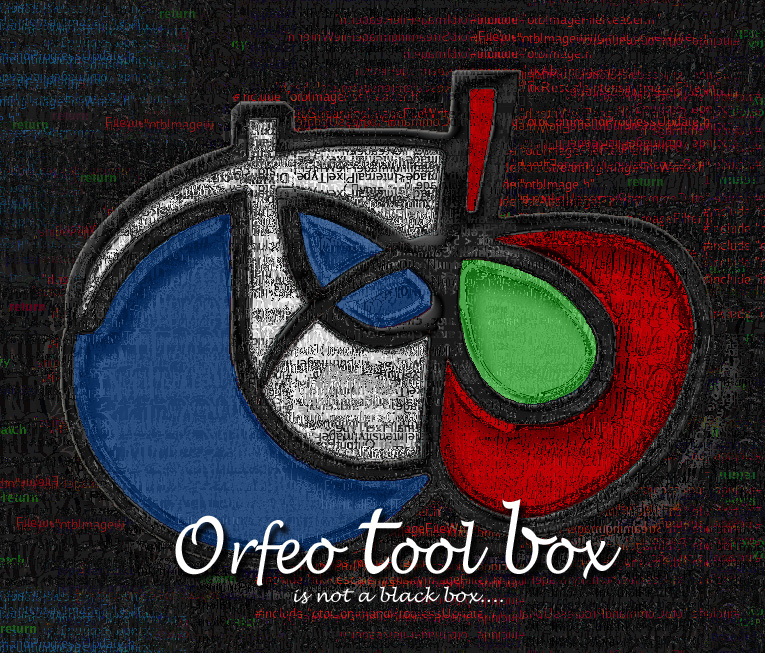
\includegraphics[width=0.9\textwidth]{images/LOGOTB_blackbox.png}
\end{columns}
\begin{center}
{\huge \color{red}{Orfeo ToolBox is not a black box \ldots}}

Let's start by opening the box!
\end{center}

\end{frame}

\begin{frame}
\frametitle{Things to know about OTB\ldots}
\begin{block}{The Orfeo ToolBox is:}
\begin{itemize}
\item A (The) \textbf{image processing library} dedicated to remote sensing,
\item \textbf{Free and open source software} under CeCILL-v2 license(equivalent to GPL),
\item \textbf{Funded and developed by CNES (French Space Agency)} in the frame
  of the ORFEO Pléiade program Orfeo (and beyond),
\item Written in \textbf{C++} on top of \href{www.itk.org}{ITK} (medical image
  processing),
\item Interfaces seamlessly with other IP and RS open-source software, like GDAL, OSSIM, OpenCV \ldots
\item Conçue pour traiter de \textbf{gros volumes de données} de manière
  transparente grâce au traitement par morceaux et à la parallélisation.
\item Concue to process \textbf{large data} thanks to parallel and on the flow processing
\end{itemize}
\end{block}

\begin{center}
{\huge\textcolor{red}{www.orfeo-toolbox.org}}
\end{center}

\end{frame}

\section{Back in 2006\ldots}

\begin{frame}
\frametitle{How it starts?}

\begin{block}{CNES Orfeo accompaniement program (2006-2014)}
\begin{itemize}
\item Constat: Le saut en résolution spatial de Pléiades par rapport à SPOT5 conduit à de nouveaux usages
\item Goals: prepare, accompany and promote the use and the exploitation of the images derived from Pléiades satellites (and CosmoSkymed)
\item Preparatory phase from 2006 to 2012,
\item Thematic Commissioning activities from 2012 to 2014.
\end{itemize}
\end{block}

\begin{block}{OTB in the Orfeo program}
\begin{itemize}
\item Answer to ORFEO user groups needs
\item Capitalize CNES R\&D in extraction of information
\item Deliver generic tools for Pleiades users
\end{itemize}
\end{block}
\end{frame}

\begin{frame}[fragile]
\frametitle{Why is it Open source?}

\begin{block}{Diffusion maximale}
Image processing library dedicated to remote sensing for Pleaides users.Its wide
dissemination contributes to the mission valorization.
\end{block}

\begin{block}{Quality and powerful}
OTB covers a vast panel of applciations and domains. Openess allows:
\begin{itemize}
\item Facilitate appropriation and validation for users,
\item Encourage contributions and bug reports,
\item Available on multiple platforms
\item The Cathedral and the Bazaar
\end{itemize}
\end{block}

\begin{block}{Reproducible research}
OTB capitalizes a part of the CNES R\&D in IP, open source contributes to  transparent, reproducible and transdisciplinary research.
\end{block}

\end{frame}

\begin{frame}
\frametitle{History \ldots}


\begin{chronology}[2]{2006}{2014}{\textwidth}
\event{\decimaldate{30}{06}{2006}}{\small{\textbf{1.0.0}}}
\end{chronology}

\begin{minipage}[t][6cm][t]{\textwidth}
\begin{block}{Key steps}
\begin{description}
\item[1.0.0] Architecture, compilation and documentation, few functions and applications
\end{description}
\end{block}
\end{minipage}
\end{frame}

\begin{frame}
\frametitle{OTB history \ldots}

\begin{chronology}[2]{2006}{2014}{\textwidth}
\event{\decimaldate{14}{12}{2007}}{\small{\textbf{2.0.0}}}
\event{\decimaldate{24}{10}{2007}}{\tiny{1.6.0}}
\event{\decimaldate{05}{06}{2007}}{\tiny{1.4.0}}
\event{\decimaldate{28}{02}{2007}}{\tiny{1.2.0}}
\event{\decimaldate{30}{06}{2006}}{\small{\textbf{1.0.0}}}
\end{chronology}

\begin{minipage}[t][6cm][t]{\textwidth}
\begin{block}{Key steps}
\begin{description}
\item[1.0.0] Architecture, compilation and documentation, few functions and applications
\item[2.0.0] More functions (SVM learning, feature extraction, pre-processing, vizualization \ldots)
\end{description}
\end{block}
\end{minipage}
\end{frame}


\begin{frame}
\frametitle{OTB history\ldots}

\begin{chronology}[2]{2006}{2014}{\textwidth}
\event{\decimaldate{15}{05}{2009}}{\small{\textbf{3.0.0}}}
\event{\decimaldate{16}{01}{2009}}{\tiny{2.8}}
\event{\decimaldate{31}{10}{2008}}{\tiny{2.6.0}}
\event{\decimaldate{29}{07}{2008}}{\tiny{2.4.0}}
\event{\decimaldate{30}{05}{2008}}{\tiny{2.2.0}}
\event{\decimaldate{14}{12}{2007}}{\small{\textbf{2.0.0}}}
\event{\decimaldate{24}{10}{2007}}{\tiny{1.6.0}}
\event{\decimaldate{05}{06}{2007}}{\tiny{1.4.0}}
\event{\decimaldate{28}{02}{2007}}{\tiny{1.2.0}}
\event{\decimaldate{30}{06}{2006}}{\small{\textbf{1.0.0}}}
\end{chronology}

\begin{minipage}[t][6cm][t]{\textwidth}
\begin{block}{Key steps}
\begin{description}
\item[1.0.0] Architecture, compilation and documentation, few functions and applications
\item[2.0.0] More functions (SVM learning, feature extraction, pre-processing, vizualization \ldots)
\item[3.0.0] Support for vector data, Markov Random Field, keypoints, Kohonen
  map  \ldots) and more applications for demonstration (with GUI)
\end{description}
\end{block}
\end{minipage}
\end{frame}


\begin{frame}
\frametitle{OTB history \ldots}

\begin{chronology}[2]{2006}{2014}{\textwidth}
\event{\decimaldate{22}{01}{2010}}{\tiny{3.2.0}}
\event{\decimaldate{15}{05}{2009}}{\small{\textbf{3.0.0}}}
\event{\decimaldate{16}{01}{2009}}{\tiny{2.8}}
\event{\decimaldate{31}{10}{2008}}{\tiny{2.6.0}}
\event{\decimaldate{29}{07}{2008}}{\tiny{2.4.0}}
\event{\decimaldate{30}{05}{2008}}{\tiny{2.2.0}}
\event{\decimaldate{14}{12}{2007}}{\small{\textbf{2.0.0}}}
\event{\decimaldate{24}{10}{2007}}{\tiny{1.6.0}}
\event{\decimaldate{05}{06}{2007}}{\tiny{1.4.0}}
\event{\decimaldate{28}{02}{2007}}{\tiny{1.2.0}}
\event{\decimaldate{30}{06}{2006}}{\small{\textbf{1.0.0}}}
\end{chronology}

\begin{minipage}[t][6cm][t]{\textwidth}
\begin{block}{Key steps}
\begin{description}
\item[1.0.0] Architecture, compilation and documentation, few functions and applications
\item[2.0.0] More functions (SVM learning, feature extraction, pre-processing, vizualization \ldots)
\item[3.0.0] Support for vector data, Markov Random Field, keypoints, Kohonen
  map  \ldots) and more applications for demonstration (with GUI)
\item[3.2.0] First version of Monteverdi, continue to enrich the library

\end{description}
\end{block}
\end{minipage}
\end{frame}

\begin{frame}
\frametitle{History \ldots}

\begin{chronology}[2]{2006}{2014}{\textwidth}
\event{\decimaldate{31}{01}{2012}}{\tiny{3.12.0}}
\event{\decimaldate{29}{06}{2011}}{\tiny{3.10.0}}
\event{\decimaldate{16}{12}{2010}}{\tiny{3.8.0}}
\event{\decimaldate{07}{10}{2010}}{\tiny{3.6.0}}
\event{\decimaldate{11}{07}{2010}}{\tiny{3.4.0}}
\event{\decimaldate{22}{01}{2010}}{\tiny{3.2.0}}
\event{\decimaldate{15}{05}{2009}}{\small{\textbf{3.0.0}}}
\event{\decimaldate{16}{01}{2009}}{\tiny{2.8}}
\event{\decimaldate{31}{10}{2008}}{\tiny{2.6.0}}
\event{\decimaldate{29}{07}{2008}}{\tiny{2.4.0}}
\event{\decimaldate{30}{05}{2008}}{\tiny{2.2.0}}
\event{\decimaldate{14}{12}{2007}}{\small{\textbf{2.0.0}}}
\event{\decimaldate{24}{10}{2007}}{\tiny{1.6.0}}
\event{\decimaldate{05}{06}{2007}}{\tiny{1.4.0}}
\event{\decimaldate{28}{02}{2007}}{\tiny{1.2.0}}
\event{\decimaldate{30}{06}{2006}}{\small{\textbf{1.0.0}}}

\end{chronology}
\begin{minipage}[t][6cm][t]{\textwidth}
\begin{block}{\'Etapes clés}
\begin{description}
\item[1.0.0] Architecture, compilation and documentation, few functions and applications
\item[2.0.0] More functions (SVM learning, feature extraction, pre-processing, vizualization \ldots)
\item[3.0.0] Support for vector data, Markov Random Field, keypoints, Kohonen
  map  \ldots) and more applications for demonstration (with GUI)
\item[3.2.0] First version of Monteverdi, continue to enrich the library
\item[3.12.0] New applications mechanisms, complete support for Pleiades
  imagery, new functions\ldots
\end{description}
\end{block}
\end{minipage}
\end{frame}

\begin{frame}
\frametitle{History \ldots}

\begin{chronology}[2]{2006}{2014}{\textwidth}
\event{\decimaldate{01}{02}{2013}}{\tiny{3.16.0}}
\event{\decimaldate{9}{07}{2012}}{\tiny{3.14.0}}
\event{\decimaldate{31}{01}{2012}}{\tiny{3.12.0}}
\event{\decimaldate{29}{06}{2011}}{\tiny{3.10.0}}
\event{\decimaldate{16}{12}{2010}}{\tiny{3.8.0}}
\event{\decimaldate{07}{10}{2010}}{\tiny{3.6.0}}
\event{\decimaldate{11}{07}{2010}}{\tiny{3.4.0}}
\event{\decimaldate{22}{01}{2010}}{\tiny{3.2.0}}
\event{\decimaldate{15}{05}{2009}}{\small{\textbf{3.0.0}}}
\event{\decimaldate{16}{01}{2009}}{\tiny{2.8}}
\event{\decimaldate{31}{10}{2008}}{\tiny{2.6.0}}
\event{\decimaldate{29}{07}{2008}}{\tiny{2.4.0}}
\event{\decimaldate{30}{05}{2008}}{\tiny{2.2.0}}
\event{\decimaldate{14}{12}{2007}}{\small{\textbf{2.0.0}}}
\event{\decimaldate{24}{10}{2007}}{\tiny{1.6.0}}
\event{\decimaldate{05}{06}{2007}}{\tiny{1.4.0}}
\event{\decimaldate{28}{02}{2007}}{\tiny{1.2.0}}
\event{\decimaldate{30}{06}{2006}}{\small{\textbf{1.0.0}}}

\end{chronology}
\begin{minipage}[t][6cm][t]{\textwidth}
\begin{block}{\'Etapes clés}
\begin{description}
\item[1.0.0] Architecture, compilation and documentation, few functions and applications
\item[2.0.0] More functions (SVM learning, feature extraction, pre-processing, vizualization \ldots)
\item[3.0.0] Support for vector data, Markov Random Field, keypoints, Kohonen
  map  \ldots) and more applications for demonstration (with GUI)
\item[3.2.0] First version of Monteverdi, continue to enrich the library
\item[3.12.0] New applications mechanisms, complete support for Pleiades
  imagery, new functions\ldots
\item[3.16.0] Revamp of Monteverdi in \textbf{Monteverdi2}
\end{description}
\end{block}
\end{minipage}
\end{frame}

\begin{frame}
\frametitle{Un peu d'histoire \ldots}

\begin{chronology}[2]{2006}{2014}{\textwidth}
\event{\decimaldate{01}{9}{2014}}{\tiny{4.2.0}}
\event{\decimaldate{12}{03}{2014}}{\small{\textbf{4.0.0}}}
\event{\decimaldate{12}{11}{2013}}{\tiny{3.20.0}}
\event{\decimaldate{04}{07}{2013}}{\tiny{3.18.0}}
\event{\decimaldate{01}{02}{2013}}{\tiny{3.16.0}}
\event{\decimaldate{9}{07}{2012}}{\tiny{3.14.0}}
\event{\decimaldate{31}{01}{2012}}{\tiny{3.12.0}}
\event{\decimaldate{29}{06}{2011}}{\tiny{3.10.0}}
\event{\decimaldate{16}{12}{2010}}{\tiny{3.8.0}}
\event{\decimaldate{07}{10}{2010}}{\tiny{3.6.0}}
\event{\decimaldate{11}{07}{2010}}{\tiny{3.4.0}}
\event{\decimaldate{22}{01}{2010}}{\tiny{3.2.0}}
\event{\decimaldate{15}{05}{2009}}{\small{\textbf{3.0.0}}}
\event{\decimaldate{16}{01}{2009}}{\tiny{2.8}}
\event{\decimaldate{31}{10}{2008}}{\tiny{2.6.0}}
\event{\decimaldate{29}{07}{2008}}{\tiny{2.4.0}}
\event{\decimaldate{30}{05}{2008}}{\tiny{2.2.0}}
\event{\decimaldate{14}{12}{2007}}{\small{\textbf{2.0.0}}}
\event{\decimaldate{24}{10}{2007}}{\tiny{1.6.0}}
\event{\decimaldate{05}{06}{2007}}{\tiny{1.4.0}}
\event{\decimaldate{28}{02}{2007}}{\tiny{1.2.0}}
\event{\decimaldate{30}{06}{2006}}{\small{\textbf{1.0.0}}}

\end{chronology}
\begin{minipage}[t][6cm][t]{\textwidth}
\begin{block}{\'Etapes clés}
\begin{description}
\item[4.0.0] Compatible with ITK 4.0, and more functions.
\end{description}
\end{block}
\end{minipage}
\end{frame}


\begin{frame}
\frametitle{A bit of history \ldots}

\begin{chronology}[2]{2006}{2014}{\textwidth}
%2 days ago 	4.0.0
% months ago 	3.20.0 	
% months ago 	3.18.0 	
%3 months ago 	3.16.0 	
%0 months ago 	3.14.0 	
\event{\decimaldate{01}{9}{2014}}{\tiny{4.2.0}}
\event{\decimaldate{12}{03}{2014}}{\small{\textbf{4.0.0}}}
\event{\decimaldate{12}{11}{2013}}{\tiny{3.20.0}}
\event{\decimaldate{04}{07}{2013}}{\tiny{3.18.0}}
\event{\decimaldate{01}{02}{2013}}{\tiny{3.16.0}}
\event{\decimaldate{9}{07}{2012}}{\tiny{3.14.0}}
\event{\decimaldate{31}{01}{2012}}{\tiny{3.12.0}}
\event{\decimaldate{29}{06}{2011}}{\tiny{3.10.0}}
\event{\decimaldate{16}{12}{2010}}{\tiny{3.8.0}}
\event{\decimaldate{07}{10}{2010}}{\tiny{3.6.0}}
\event{\decimaldate{11}{07}{2010}}{\tiny{3.4.0}}
\event{\decimaldate{22}{01}{2010}}{\tiny{3.2.0}}
\event{\decimaldate{15}{05}{2009}}{\small{\textbf{3.0.0}}}
\event{\decimaldate{16}{01}{2009}}{\tiny{2.8}}
\event{\decimaldate{31}{10}{2008}}{\tiny{2.6.0}}
\event{\decimaldate{29}{07}{2008}}{\tiny{2.4.0}}
\event{\decimaldate{30}{05}{2008}}{\tiny{2.2.0}}
\event{\decimaldate{14}{12}{2007}}{\small{\textbf{2.0.0}}}
\event{\decimaldate{24}{10}{2007}}{\tiny{1.6.0}}
\event{\decimaldate{05}{06}{2007}}{\tiny{1.4.0}}
\event{\decimaldate{28}{02}{2007}}{\tiny{1.2.0}}
\event{\decimaldate{30}{06}{2006}}{\small{\textbf{1.0.0}}}

\end{chronology}

\begin{minipage}[t][6cm][t]{\textwidth}
\begin{block}{Lines of code}
\begin{center}
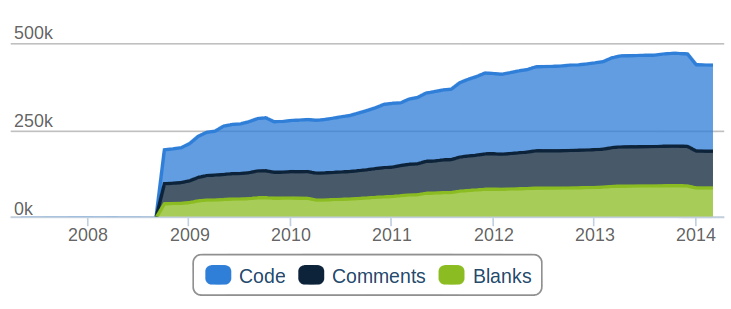
\includegraphics[width=\textwidth]{images/lines_of_code_crop.png}
\end{center}
\end{block}
\end{minipage}

\end{frame}


\begin{frame}
\frametitle{A bit of history \ldots}

\begin{chronology}[2]{2006}{2014}{\textwidth}
%2 days ago 	4.0.0
% months ago 	3.20.0 	
% months ago 	3.18.0 	
%3 months ago 	3.16.0 	
%0 months ago 	3.14.0 	
\event{\decimaldate{01}{9}{2014}}{\tiny{4.2.0}}
\event{\decimaldate{12}{03}{2014}}{\small{\textbf{4.0.0}}}
\event{\decimaldate{12}{11}{2013}}{\tiny{3.20.0}}
\event{\decimaldate{04}{07}{2013}}{\tiny{3.18.0}}
\event{\decimaldate{01}{02}{2013}}{\tiny{3.16.0}}
\event{\decimaldate{9}{07}{2012}}{\tiny{3.14.0}}
\event{\decimaldate{31}{01}{2012}}{\tiny{3.12.0}}
\event{\decimaldate{29}{06}{2011}}{\tiny{3.10.0}}
\event{\decimaldate{16}{12}{2010}}{\tiny{3.8.0}}
\event{\decimaldate{07}{10}{2010}}{\tiny{3.6.0}}
\event{\decimaldate{11}{07}{2010}}{\tiny{3.4.0}}
\event{\decimaldate{22}{01}{2010}}{\tiny{3.2.0}}
\event{\decimaldate{15}{05}{2009}}{\small{\textbf{3.0.0}}}
\event{\decimaldate{16}{01}{2009}}{\tiny{2.8}}
\event{\decimaldate{31}{10}{2008}}{\tiny{2.6.0}}
\event{\decimaldate{29}{07}{2008}}{\tiny{2.4.0}}
\event{\decimaldate{30}{05}{2008}}{\tiny{2.2.0}}
\event{\decimaldate{14}{12}{2007}}{\small{\textbf{2.0.0}}}
\event{\decimaldate{24}{10}{2007}}{\tiny{1.6.0}}
\event{\decimaldate{05}{06}{2007}}{\tiny{1.4.0}}
\event{\decimaldate{28}{02}{2007}}{\tiny{1.2.0}}
\event{\decimaldate{30}{06}{2006}}{\small{\textbf{1.0.0}}}

\end{chronology}
\begin{minipage}[t][6cm][t]{\textwidth}
\begin{block}{Commits per month}
\begin{center}
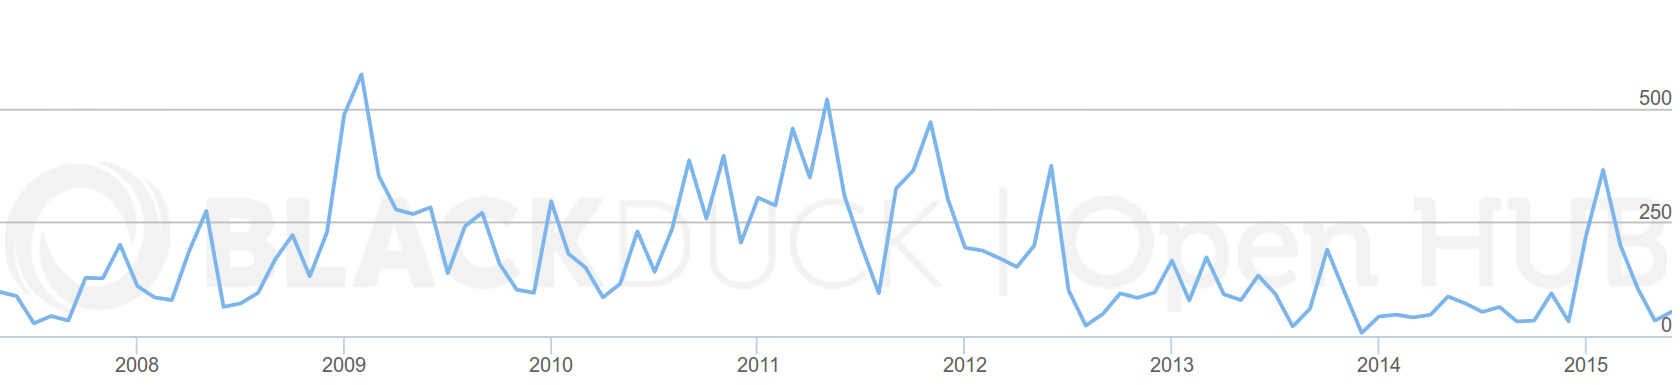
\includegraphics[width=\textwidth]{images/commits_per_month_crop.png}
\end{center}
\end{block}
\end{minipage}
\end{frame}

\begin{frame}
\frametitle{A bit of history \ldots}

\begin{chronology}[2]{2006}{2014}{\textwidth}
%2 days ago 	4.0.0
% months ago 	3.20.0 	
% months ago 	3.18.0 	
%3 months ago 	3.16.0 	
%0 months ago 	3.14.0 	
\event{\decimaldate{4}{9}{2014}}{\tiny{4.2.0}}
\event{\decimaldate{12}{03}{2014}}{\small{\textbf{4.0.0}}}
\event{\decimaldate{12}{11}{2013}}{\tiny{3.20.0}}
\event{\decimaldate{04}{07}{2013}}{\tiny{3.18.0}}
\event{\decimaldate{01}{02}{2013}}{\tiny{3.16.0}}
\event{\decimaldate{9}{07}{2012}}{\tiny{3.14.0}}
\event{\decimaldate{31}{01}{2012}}{\tiny{3.12.0}}
\event{\decimaldate{29}{06}{2011}}{\tiny{3.10.0}}
\event{\decimaldate{16}{12}{2010}}{\tiny{3.8.0}}
\event{\decimaldate{07}{10}{2010}}{\tiny{3.6.0}}
\event{\decimaldate{11}{07}{2010}}{\tiny{3.4.0}}
\event{\decimaldate{22}{01}{2010}}{\tiny{3.2.0}}
\event{\decimaldate{15}{05}{2009}}{\small{\textbf{3.0.0}}}
\event{\decimaldate{16}{01}{2009}}{\tiny{2.8}}
\event{\decimaldate{31}{10}{2008}}{\tiny{2.6.0}}
\event{\decimaldate{29}{07}{2008}}{\tiny{2.4.0}}
\event{\decimaldate{30}{05}{2008}}{\tiny{2.2.0}}
\event{\decimaldate{14}{12}{2007}}{\small{\textbf{2.0.0}}}
\event{\decimaldate{24}{10}{2007}}{\tiny{1.6.0}}
\event{\decimaldate{05}{06}{2007}}{\tiny{1.4.0}}
\event{\decimaldate{28}{02}{2007}}{\tiny{1.2.0}}
\event{\decimaldate{30}{06}{2006}}{\small{\textbf{1.0.0}}}

\end{chronology}
\begin{minipage}[t][6cm][t]{\textwidth}
\begin{block}{Sourceforge downloads}
\begin{center}
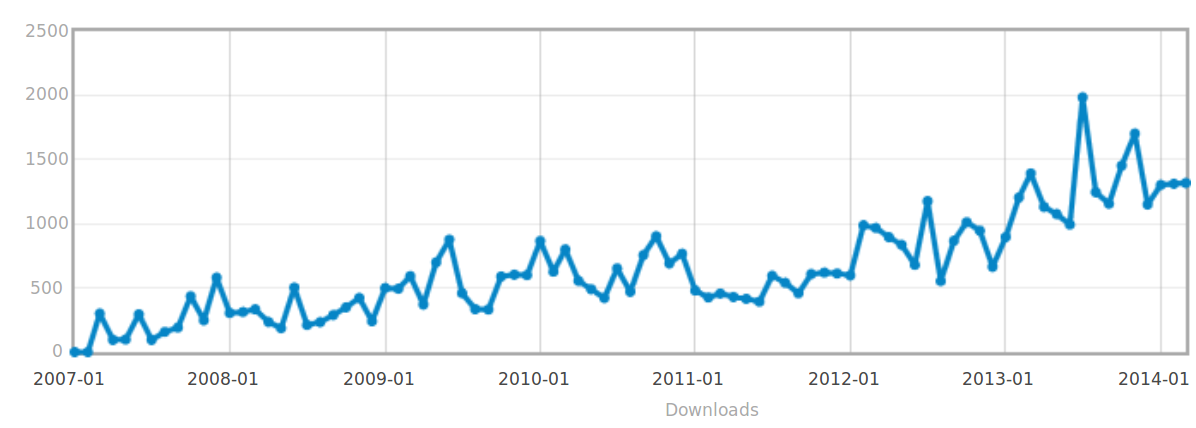
\includegraphics[width=\textwidth]{images/OTB_downloads_sourceforge.png}
\end{center}
\end{block}
\end{minipage}
\end{frame}

\section{Caractéristiques clés}

\begin{frame}
\frametitle{Construite sur des logiciels libres tiers performants}
\begin{block}{Motivations}
\begin{itemize}
\item Interfaces seamlessly with other IP and RS open-source software\ldots
\item Cette position d'intégrateur permet d'accroître rapidement le nombre de fonctions tout en assurant leurs validité
\item Combine tools to create hybrid processing chain
\end{itemize} 
\end{block}

\begin{block}{OTb backbone}
\begin{itemize}
\item \href{www.itk.org}{ITK} data processing schema based on ITK \emph{pipeline}
\item \href{www.gdal.org}{GDAL} to read/write raster/vector data,
\item \href{www.ossim.org}{OSSIM} sensor modelling and metadata support, 
\item \href{www.opencv.org}{OpenCV} et \href{www.libsvm.org}{LibSVM} provide
  machine learning algorithms,
\item \href{www.muparser.org}{MuParser} et \href{www.muparserx.org}{MuParserX}
  powerful parsing of mathematical expression (band math)\ldots
\end{itemize}
\end{block}


\end{frame}

\begin{frame}
\frametitle{Compatible (and available) on multiple plateforms}
\begin{columns}
\column{0.5\textwidth}
\begin{block}{Goal}
\begin{itemize}
\item Compile with recent versions of:
\begin{itemize}
\item gcc,
\item clang,
\item mingw
\item visual studio\ldots
\end{itemize}
\item Binary packages available:
\begin{itemize}
\item Ubuntugis repository (GIS and IP software for Ubuntu),
\item Experimental Debian packages 
\item Available in  OSGeo4W (OSGeo tools on Windows),
\item Binary installers and Port for Mac OSX\ldots
\end{itemize}
\end{itemize}
\end{block}
\column{0.5\textwidth}
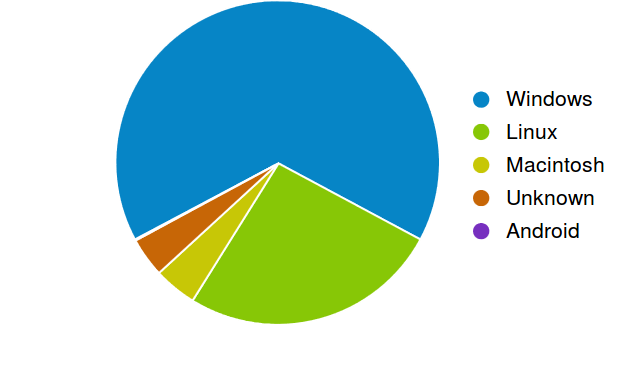
\includegraphics[width=\textwidth]{images/OTB4_download_sourceforge_os_crop.png}
\begin{center}
\tiny{OS of users which download OTB on Sourceforge}
\end{center}
\end{columns}
\end{frame}

\begin{frame}
\frametitle{Flexibility, scalability: \textit{Pipeline}, \textit{Streaming} et \textit{multithreading}}

\begin{block}{\textit{Pipeline} data model}
\begin{center}
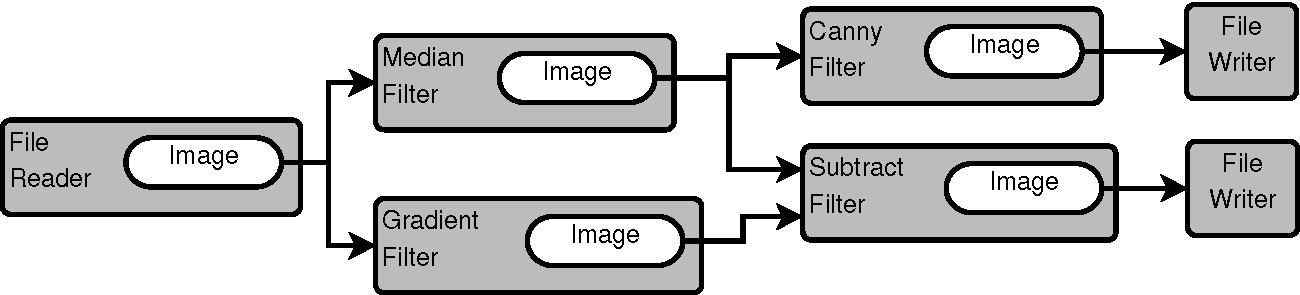
\includegraphics[width=0.7\textwidth]{images/ProcessObjectDataObject.png}
\end{center}
\end{block}
\vspace{-0.5cm}
\begin{block}{\textit{Streaming}}
\begin{center}
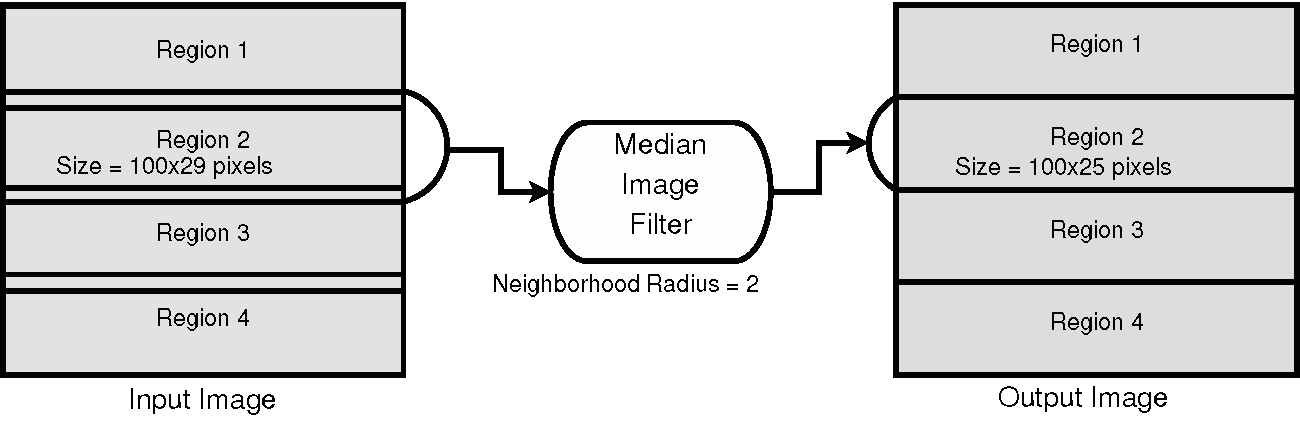
\includegraphics[width=0.7\textwidth]{images/StreamingImageDiagram.png}
\end{center}
\end{block}
\vspace{-0.5cm}
\begin{center}
\tiny{source: http://www.aosabook.org/en/itk.html}
\end{center}
\end{frame}

\begin{frame}
\frametitle{Scalability backstage \dots}
\begin{center}
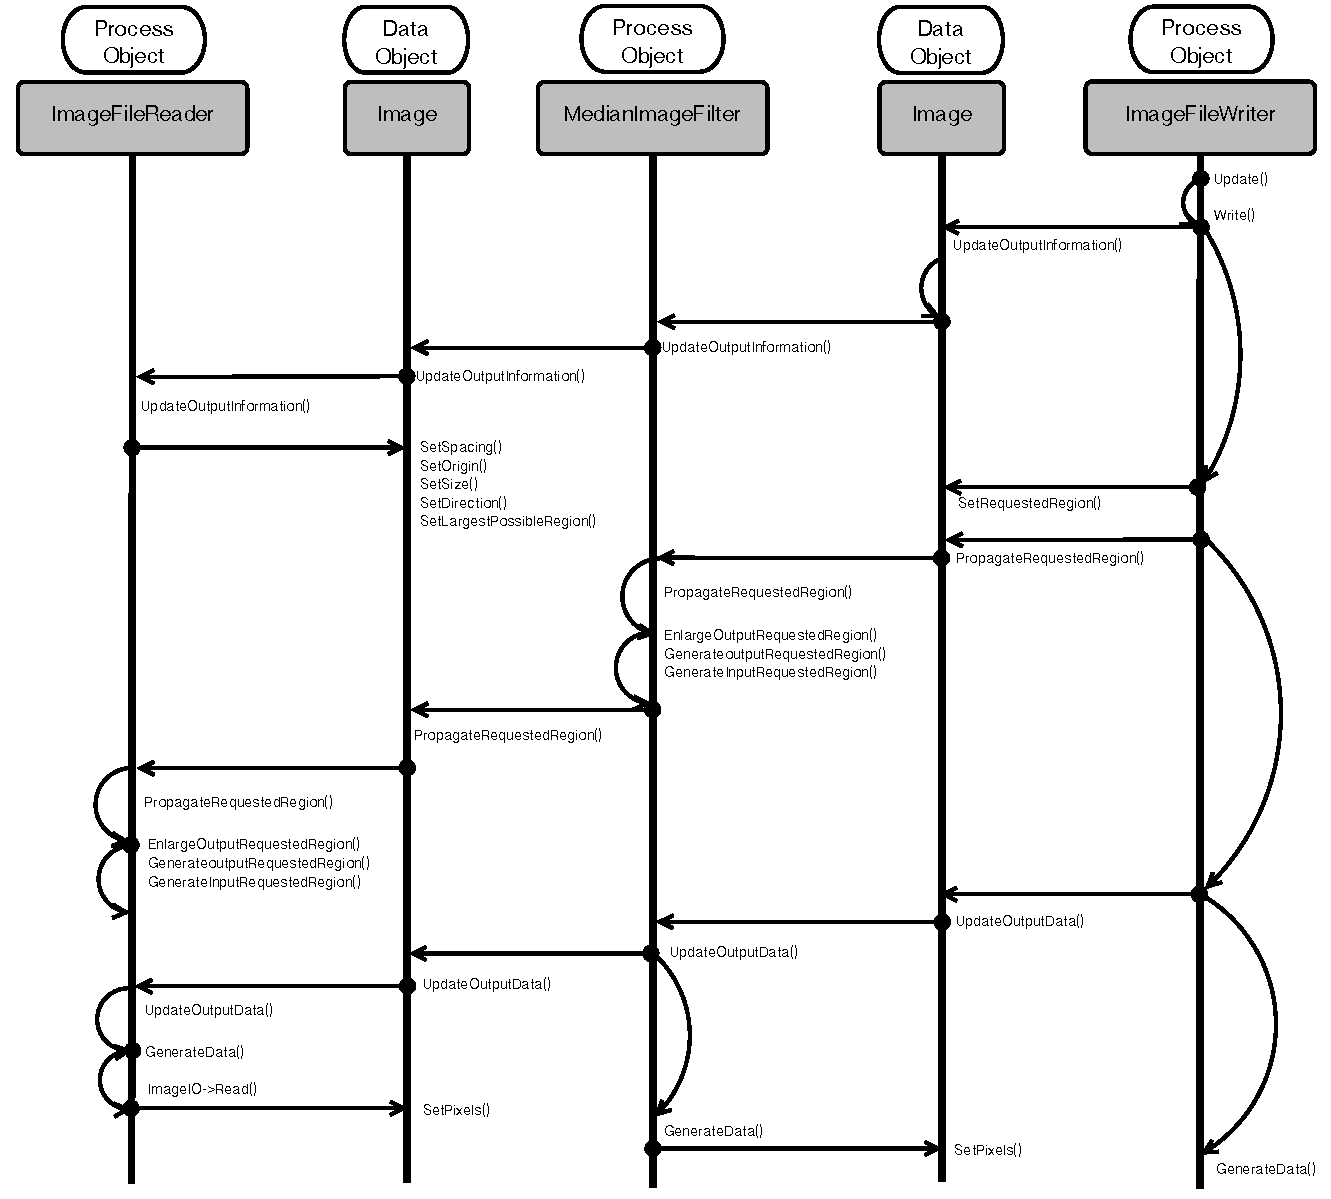
\includegraphics[width=0.6\textwidth]{images/ProcessObjectDataObjectInteractionUML.png}\\
\tiny{source: http://www.aosabook.org/en/itk.html}
\end{center}
\end{frame}

\begin{frame}
\frametitle{(Near) bleeding-edge techniques}
\begin{itemize}
\item Technology intelligence of the development team
\item Reference implementation of algorithms based on publications. e.g.:
  morphological profil, MeanShift segmentation, Haralick textures, SURF keypoints \ldots
\item Reference implementation contributes by authors with their
  publications. Ex.: Large Scale MeanShift, bayesian fusion, object detection \ldots
\item Veille pour bénéficier des avancées des logiciels tiers. e.g.:
  \textit{machine learning} module in OpenCV,
\end{itemize}
\end{frame}

\begin{frame}
\frametitle{How OTB is develop?}
\vspace{-0.5cm}
\begin{itemize}
\item Distributed version control: Mercurial (Git migration)
\item C++ and CMake (CTest, CDash)
\item Test driven development (TDD)
\item Agile (scrum)
\item Continuous integration and packaging
\end{itemize}
Every day, almost 3000 tests are compiled, launched on 16 different configurations!
\begin{center}
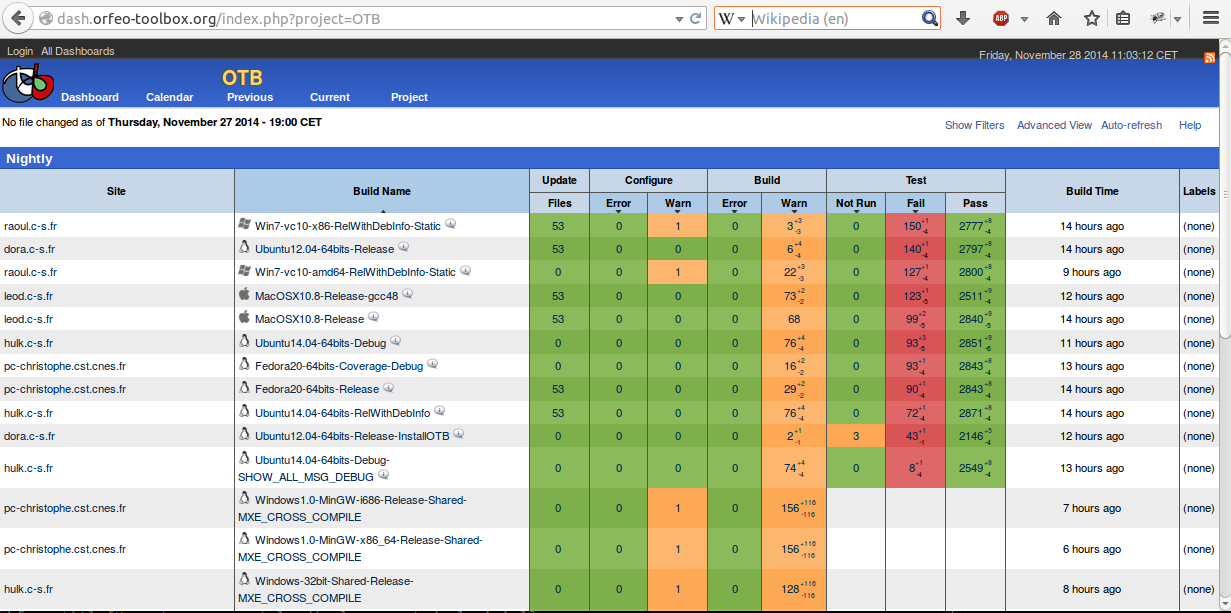
\includegraphics[width=\textwidth,trim=0 250 0 0,clip=true]{images/dashboard.png}
\end{center}
\end{frame}

\begin{frame}
\frametitle{How to eat the OTB sandwich?}
\vspace{-0.5cm}
\begin{center}
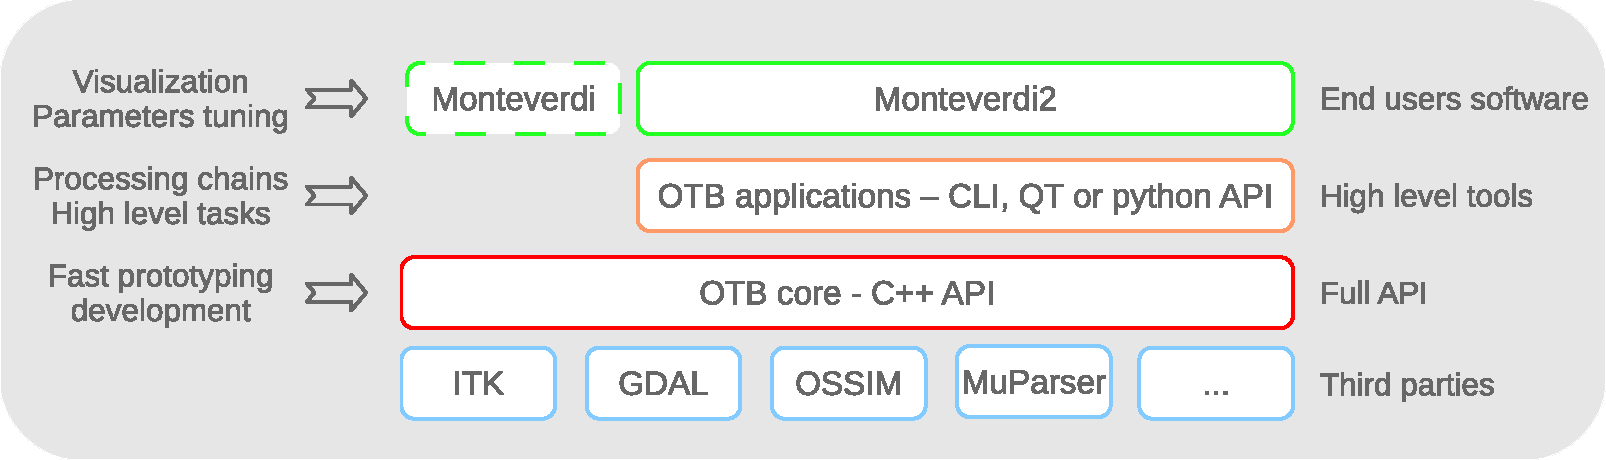
\includegraphics[width=\textwidth]{images/sandwich.pdf}
\end{center}
\vspace{-0.5cm}
\begin{block}{Write your own code}
 Flexible, access to full API, requires C++ knwoledge
\end{block}
\begin{block}{Use the applications}
 High level functions (e.g. segmentation), callable from CLI, Qt, Python, can be extended
\end{block}
\begin{block}{Use Monteverdi2}
Visualization, data management, \textcolor{red}{Access to all applications}
\end{block}
\end{frame}

\begin{frame}
\frametitle{The applications: write it once, use everywhere}
\begin{columns}
\column{0.5\textwidth}
\begin{itemize}
\item 75 applications are shipped with OTB
\item 1 application $=$ 1 dynamic library (plugin)
\item Applications are auto-descriptive and auto-documented
\item Applications can be extended outside of OTB
\item Several plugins players:
\begin{itemize}
  \item Command-line
  \item Qt auto-generated
  \item Python
\end{itemize}
\item Applications are meant for integration in external systems
\end{itemize}
\column{0.5\textwidth}
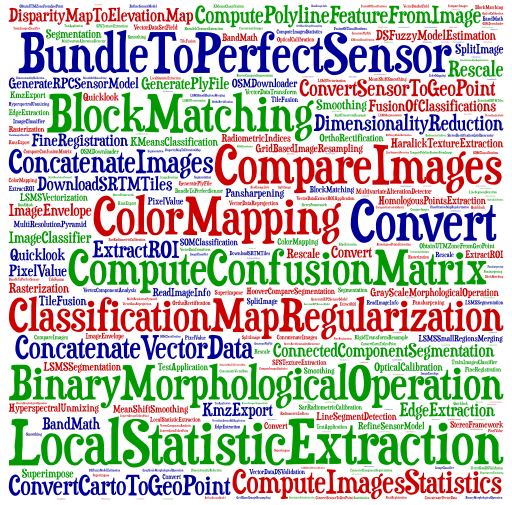
\includegraphics[width=\textwidth]{images/cloud_applications.png}
\end{columns}
\end{frame}



\begin{frame}[fragile]
\frametitle{Applications: command-line invocation}
\begin{scriptsize}
\vspace{-0.5cm}\begin{verbatim}
$ otbcli_OrthoRectification 

ERROR: Waiting for at least one parameter...
This is the OrthoRectification application, version 5.0.0
This application allows to ortho-rectify optical images from supported sensors.

Complete documentation: http://www.orfeo-toolbox.org/Applications/OrthoRectification.html

Parameters: 
        -progress                <boolean>        Report progress 
MISSING -io.in                   <string>         Input Image  (mandatory)
MISSING -io.out                  <string> [pixel] Output Image  [pixel=uint8/uint16/int16/uint32/int32/float/double] (default value is float) (mandatory)
        -map                     <string>         Output Cartographic Map Projection [utm/lambert2/lambert93/wgs/epsg] (mandatory, default value is utm)
        -map.utm.zone            <int32>          Zone number  (mandatory, default value is 31)
        -map.utm.northhem        <boolean>        Northern Hemisphere  (optional, off by default)
        -map.epsg.code           <int32>          EPSG Code  (mandatory, default value is 4326)
        -outputs.mode            <string>         Parameters estimation modes [auto/autosize/autospacing/outputroi/orthofit] (mandatory, default value is auto)
MISSING -outputs.ulx             <float>          Upper Left X  (mandatory)
MISSING -outputs.uly             <float>          Upper Left Y  (mandatory)
MISSING -outputs.sizex           <int32>          Size X  (mandatory)
MISSING -outputs.sizey           <int32>          Size Y  (mandatory)
MISSING -outputs.spacingx        <float>          Pixel Size X  (mandatory)
MISSING -outputs.spacingy        <float>          Pixel Size Y  (mandatory)
        -outputs.lrx             <float>          Lower right X  (optional, off by default)
        -outputs.lry             <float>          Lower right Y  (optional, off by default)
        -outputs.ortho           <string>         Model ortho-image  (optional, off by default)
        -outputs.isotropic       <boolean>        Force isotropic spacing by default  (optional, on by default)
        -outputs.default         <float>          Default pixel value  (optional, on by default, default value is 0)
        -elev.dem                <string>         DEM directory  (optional, off by default)
        -elev.geoid              <string>         Geoid File  (optional, off by default)
        -elev.default            <float>          Default elevation  (mandatory, default value is 0)
        -interpolator            <string>         Interpolation [bco/nn/linear] (mandatory, default value is bco)
\end{verbatim}
\end{scriptsize}
\end{frame}


\begin{frame}[fragile]
\frametitle{Applications: auto-generated Qt invocation (parameters)}
\begin{center}
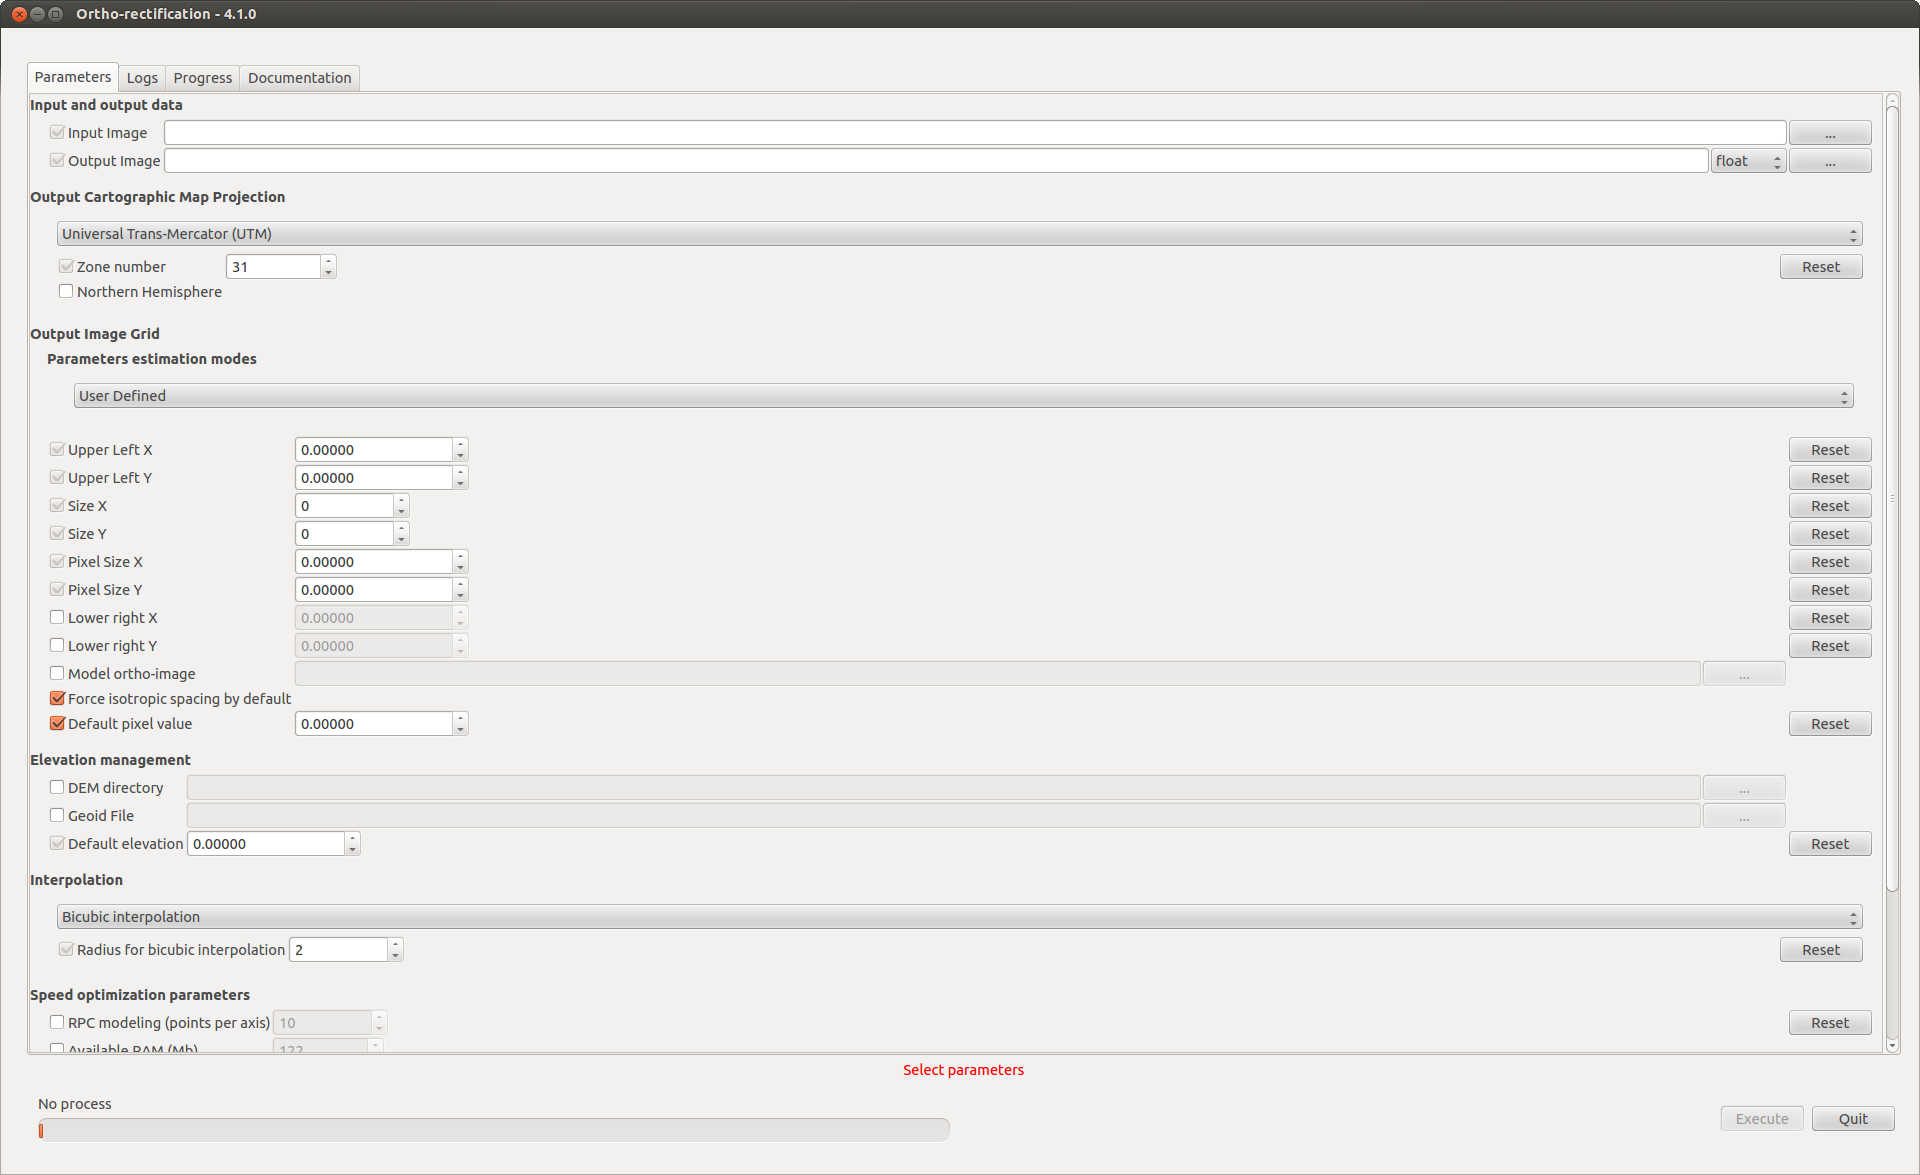
\includegraphics[width=0.9\textwidth]{images/app_parameters.png}
\end{center}
\end{frame}


\begin{frame}[fragile]
\frametitle{Applications: auto-generated Qt invocation (documentation)}
\begin{center}
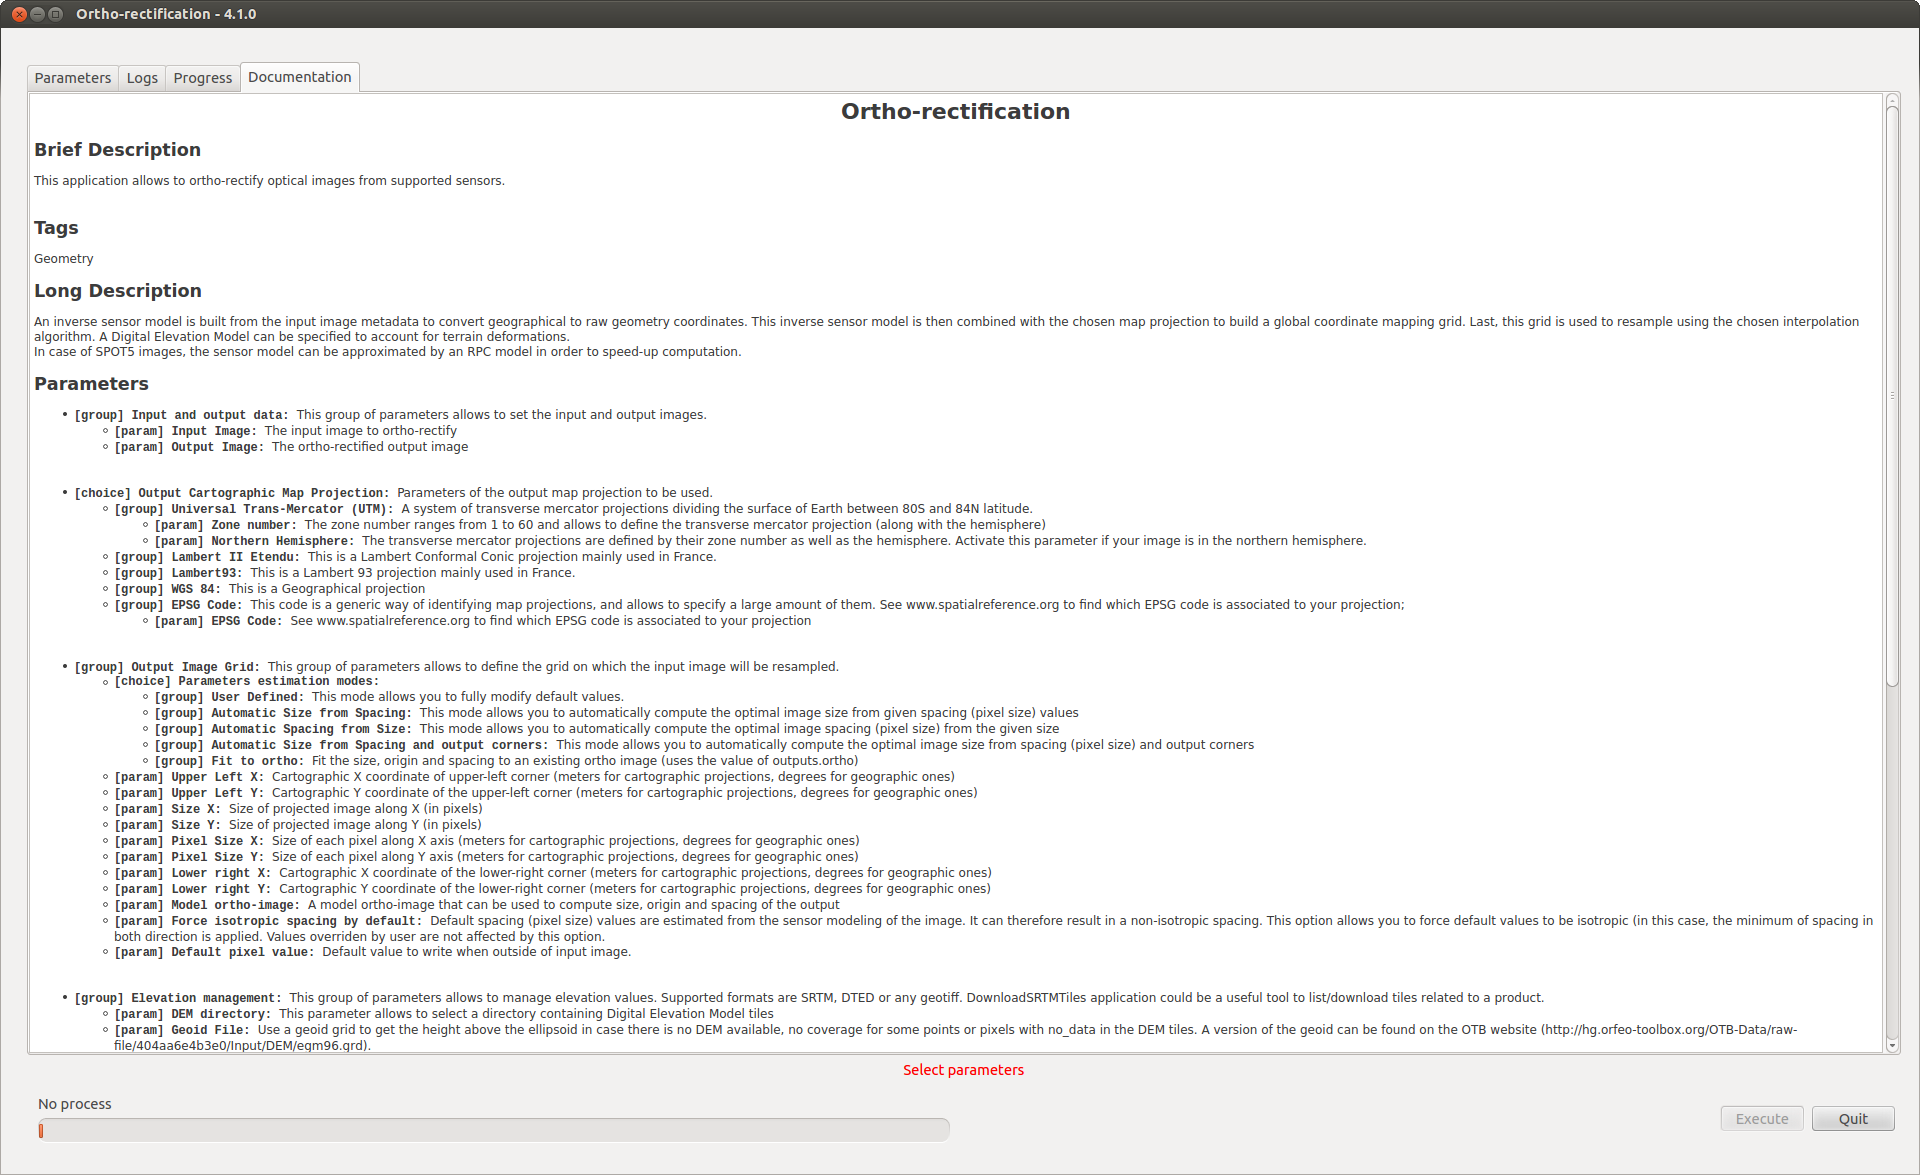
\includegraphics[width=0.9\textwidth]{images/app_doc.png}
\end{center}
\end{frame}

\begin{frame}[fragile]
\frametitle{Applications: Python wrapping}
\begin{lstlisting}[language=python,breaklines=true,breakatwhitespace=true,frame = tb,framerule = 0.25pt,fontadjust,backgroundcolor={\color{listlightgray}},basicstyle = {\ttfamily\tiny},keywordstyle = {\ttfamily\color{listkeyword}\textbf},identifierstyle = {\ttfamily},commentstyle = {\ttfamily\color{listcomment}\textit},stringstyle = {\ttfamily},showstringspaces = false,showtabs = false,numbers = none,numbersep = 6pt, numberstyle={\ttfamily\color{listnumbers}},tabsize = 2]
#!/usr/bin/python 
 
# Import the otb applications package 
import otbApplication 
 
# The following line creates an instance of the OrthoRectification application 
OrthoRectification = otbApplication.Registry.CreateApplication("OrthoRectification") 
 
# The following lines set all the application parameters: 
OrthoRectification.SetParameterString("io.in", "QB_TOULOUSE_MUL_Extract_500_500.tif") 
 
OrthoRectification.SetParameterString("io.out", "QB_Toulouse_ortho.tif") 
 
# The following line execute the application 
OrthoRectification.ExecuteAndWriteOutput()
\end{lstlisting}
\end{frame}


\begin{frame}
\frametitle{Monteverdi2: visualization}
\begin{minipage}[t][6cm][t]{\textwidth}
\begin{center}
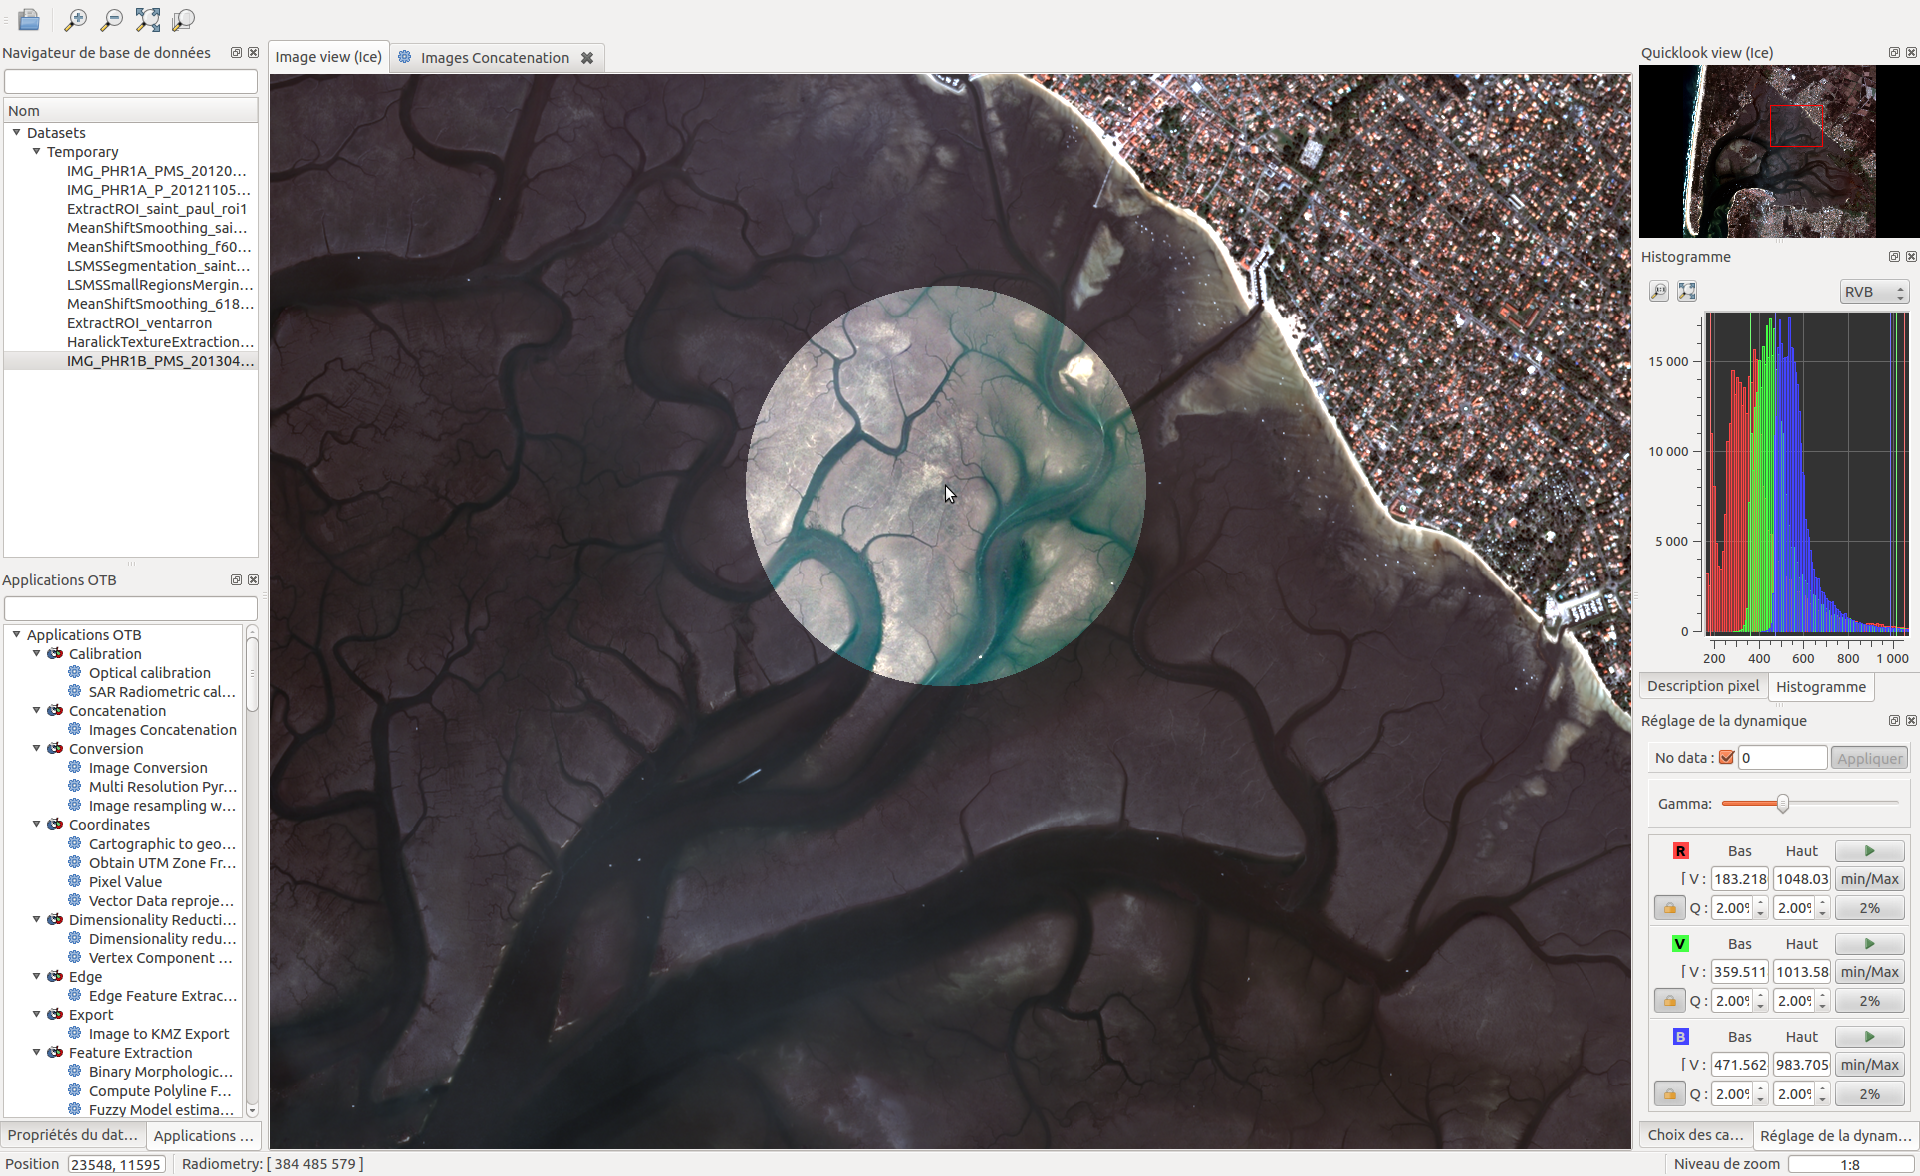
\includegraphics[width=0.9\textwidth]{images/monteverdi2-loupe.png}
\end{center}
\end{minipage}
\end{frame}
\begin{frame}

\frametitle{Monteverdi2: processing}
\begin{minipage}[t][6cm][t]{\textwidth}
\begin{center}
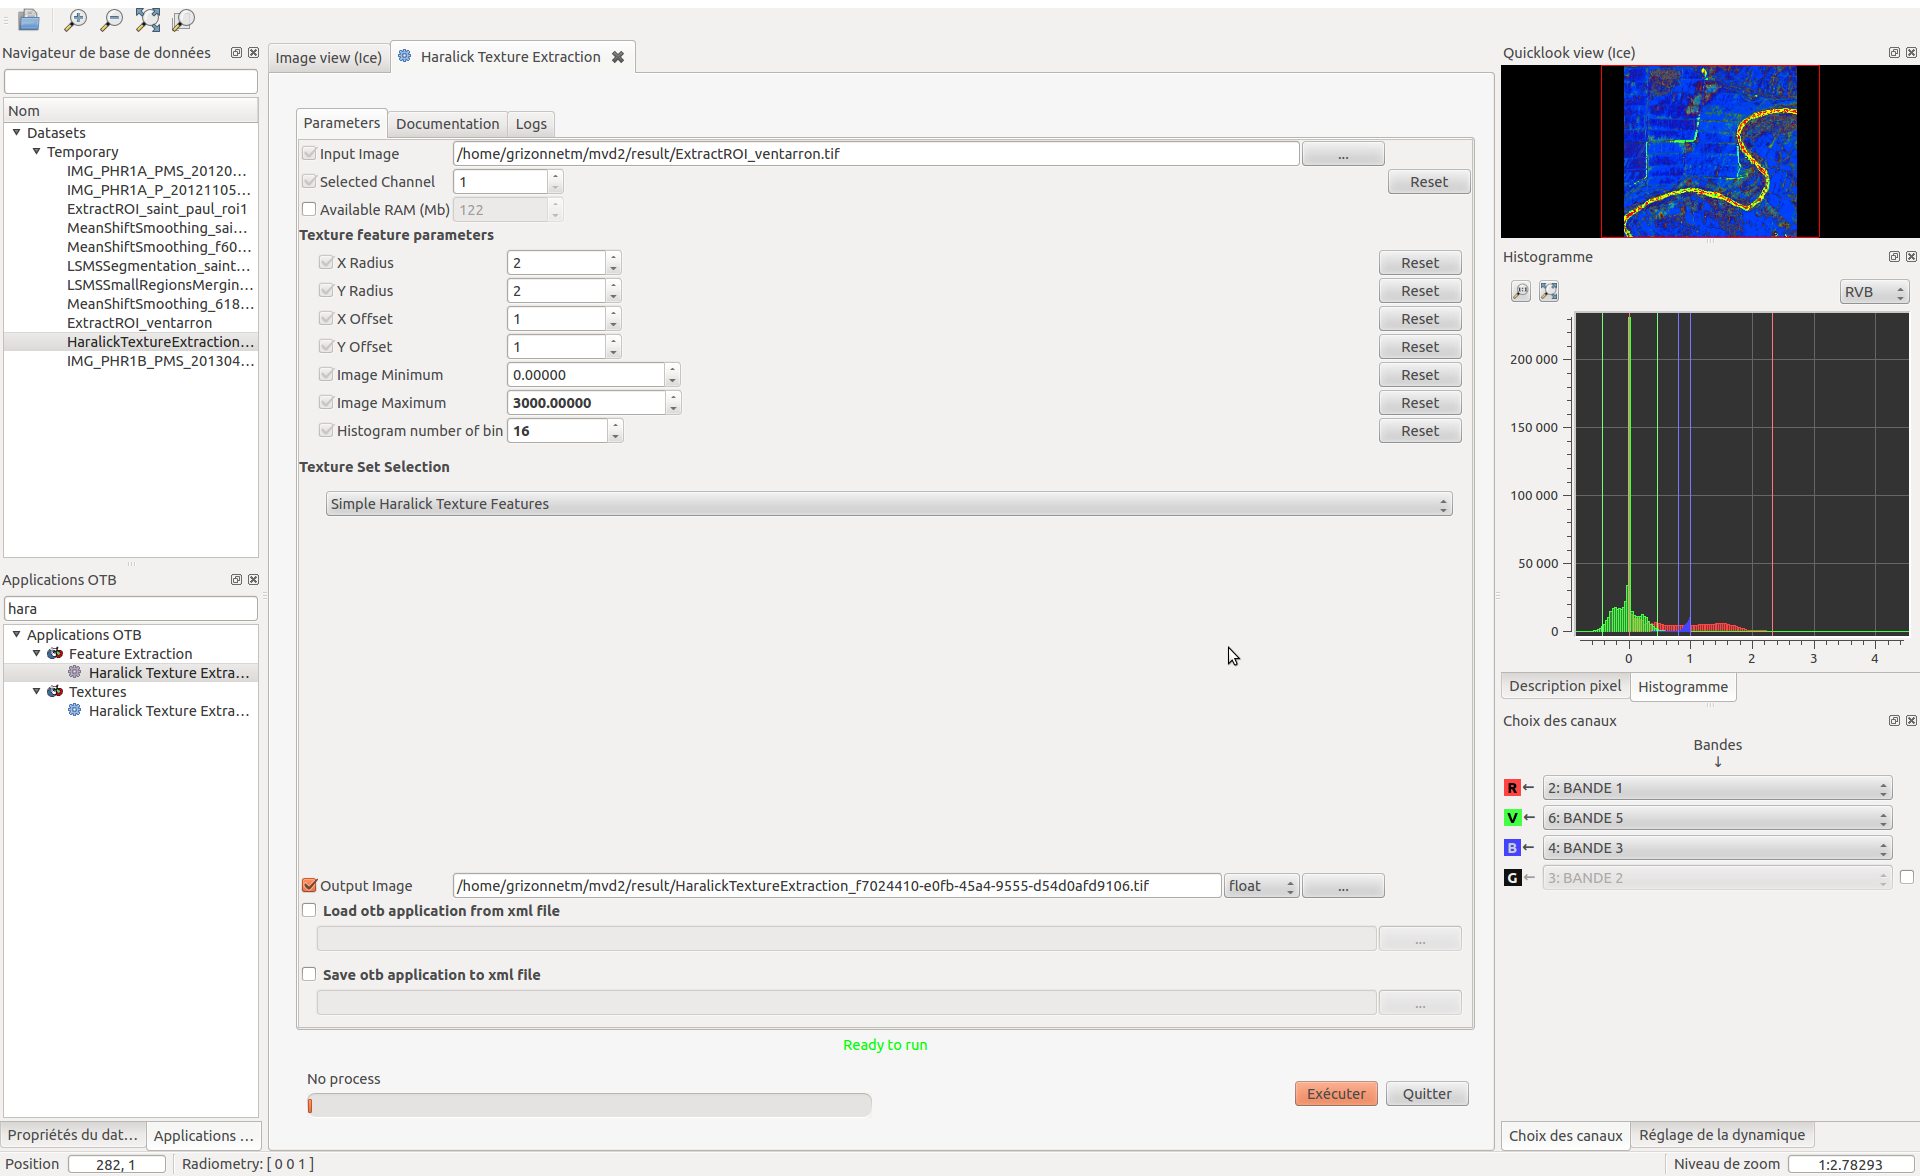
\includegraphics[width=0.9\textwidth]{images/monteverdi2-haralick.png}
\end{center}
\end{minipage}
\end{frame}


\section{Features}

\begin{frame}
\frametitle{Incomplete list of OTB functions}

\begin{block}{Pre-processing}
\begin{itemize}
\item Radiometric calibration, orthorectification, resampling (raster and
  vector), pan-sharpening, stereo rectification,
\item Sensor supported: Pléiades, SPOT6, SPOT5, DigitalGlobe satellites
\item Geometric models (thanks to OSSIM), support for DEM (SRTM or GeoTIFF)
\end{itemize}
\end{block}

\begin{block}{Images and vector manipulation}
\begin{itemize}
\item Formats supported by Gdal (raster and vector), conversion raster/vector
\item Region of interest extraction, of spectral bands, concatenation or splitting\ldots
\item Band math, color mapping, contrast enhancement
\item Linear filtering, Mathematical morphology,
\end{itemize}
\end{block}
\end{frame}

\begin{frame}
\frametitle{Incomplete list of OTB functions}

\begin{block}{Feature extraction}
\begin{itemize}
\item Edge detection, scale-invariant feature transform, lines, corners
\item Radiometric indices, textures (Haralick, SFS, PanTex)
\item Local statistics (Flusser moments, Histogram of Oriented Gradient)
\item Keypoints matching
\end{itemize}
\end{block}

\begin{block}{Change detection}
\begin{itemize}
\item Classic methods with image metrics comparaison,
\item Multivariate Alteration Detector
\end{itemize}
\end{block}

\begin{block}{Dimensionality reduction, hyperspectral processing}
\begin{itemize}
\item PCA, NAPCA, ICA, MAF \ldots
\item Dimension estimation, endmembers extraction, Vertex Component analysis (VCA)
\end{itemize}
\end{block}

\end{frame}

\begin{frame}
\frametitle{Incomplete list of OTB functions}
\begin{block}{Segmentation}
\begin{itemize}
\item Segmentation algorithms: Connected Components, MeanShift,Watershed
\item Méthods to apply those method on large dataset,
\item Vector or raster representation which allow Object Based Image Analysis
\end{itemize}
\end{block}

\begin{block}{Classification}
\begin{itemize}
\item 9 supervised methods available (including SVM and Random Forest)
\item Fusion and regularization of classifications
\item K-Means clustering or Kohonen maps
\item Object classification (from a segmentation)
\end{itemize}
\end{block}

\end{frame}

\vspace*{-6.5mm}    
\begin{frame}[plain]
\hspace*{-11mm}
    \includegraphics[keepaspectratio,height=1.1\paperheight]{images/mayotte2012.png}
\end{frame} 

\vspace*{-6.5mm}    
\begin{frame}[plain]
\hspace*{-11mm}
    \includegraphics[keepaspectratio,height=1.1\paperheight]{images/mayotte2013.png}
\end{frame} 

\vspace*{-6.5mm}    
\begin{frame}[plain]
\hspace*{-11mm}
    \includegraphics[keepaspectratio,height=1.1\paperheight]{images/mayotte_mad.png}
\end{frame} 

\vspace*{-6.5mm}    
\begin{frame}[plain]
\hspace*{-11mm}
\includegraphics[keepaspectratio,height=1.1\paperheight]{images/saint_paul_lsd.png}
\end{frame} 

\vspace*{-6.5mm}    
\begin{frame}[plain]
\hspace*{-11mm}
    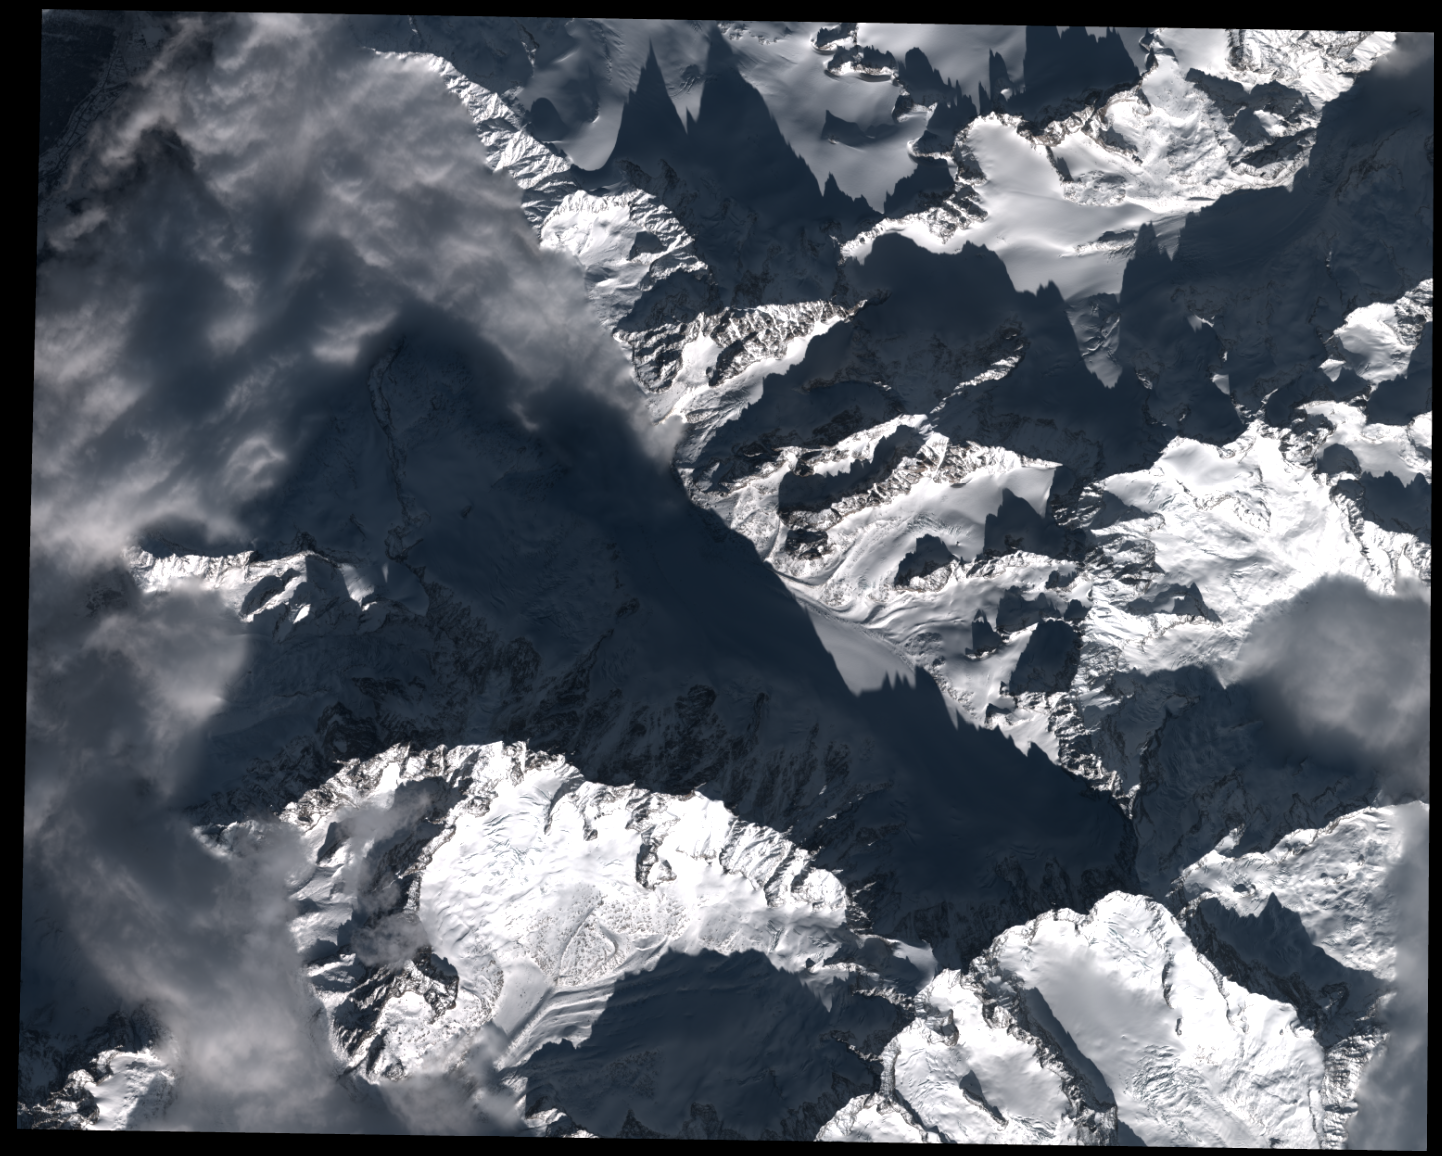
\includegraphics[keepaspectratio,width=1.005\paperwidth,height=1.1\paperheight]{images/argentiere_left.png}
\end{frame} 

\vspace*{-6.5mm}    
\begin{frame}[plain]
\hspace*{-11mm}
    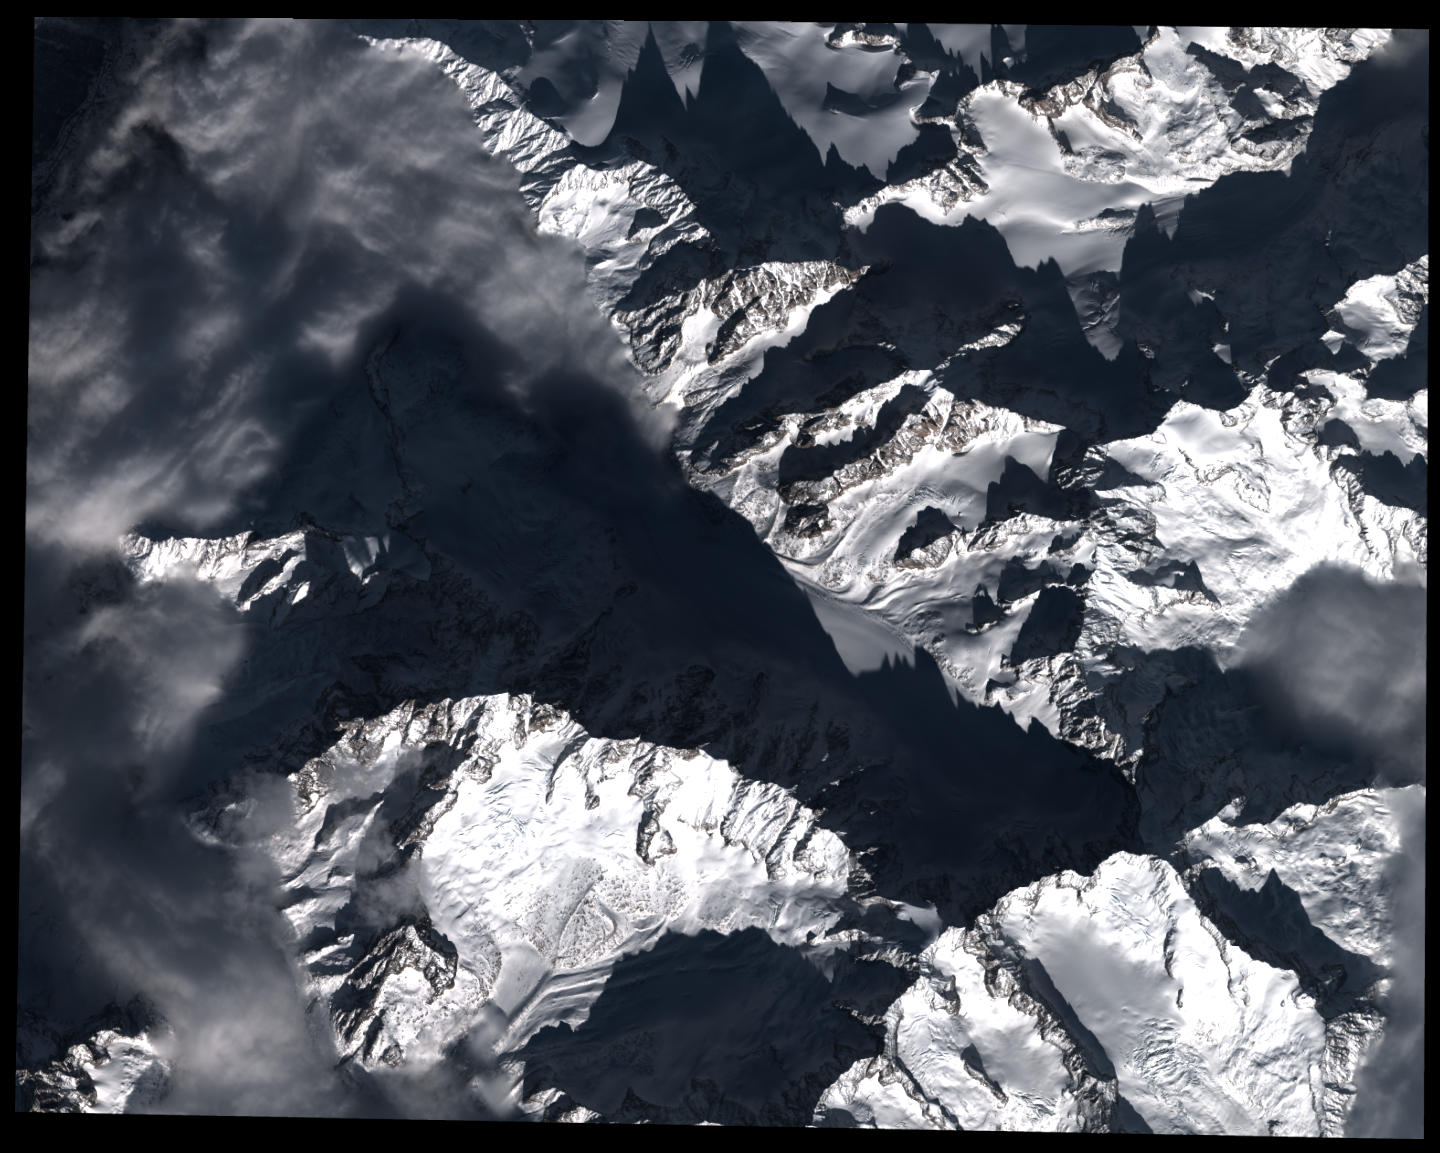
\includegraphics[keepaspectratio,width=1.005\paperwidth,height=1.1\paperheight]{images/argentiere_right.png}
\end{frame} 

\vspace*{-6.5mm}    
\begin{frame}[plain]
\hspace*{-11mm}
    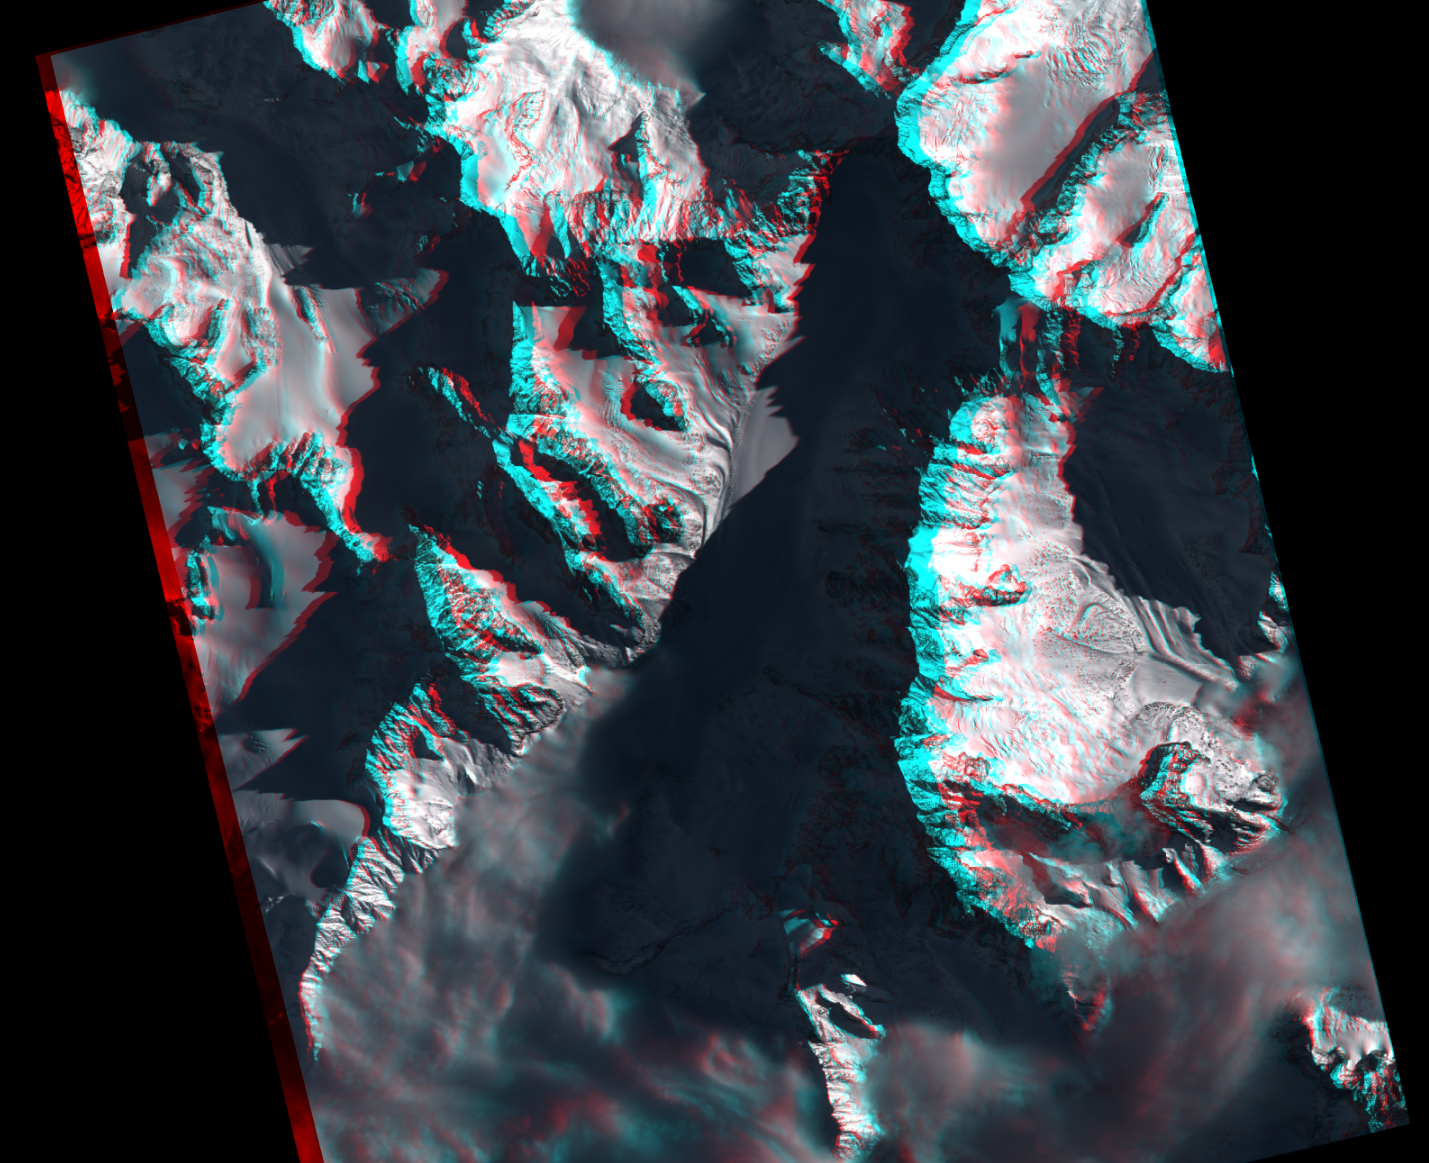
\includegraphics[keepaspectratio,width=1.005\paperwidth,height=1.1\paperheight]{images/argentiere_anaglyphe.png}
\end{frame} 

\section{What's new in OTB 5.0?}

\begin{frame}
\frametitle{Modularity (inspired by ITK 4.x)}
\begin{block}{Qu'est ce qui change?}
\begin{itemize}
\item  Organize the code into conceptual cohesive groups:
  \begin{itemize}
    \item OTB 4.4: 1672 files in 26 directories
    \item OTB 5.0: 1627 files in 124 \textbf{modules} divided in 16 groups
  \end{itemize}
\item Modules contain: tests, source code, applications are grouped
\item Each module can be (de)activate, with automatic dependencies resolutions
\end{itemize}
\end{block}

\begin{block}{Advantages?}
\begin{itemize}
\item Third part dependencies are integrated as modules and can be excluded
\item Lots of CMake magic (less code for configuration, better support)
\item Doxygen API documentation follows the new code organization (easier to
  find class info)
\item Facilitate external contributions with powerful mechanisms call \textit{remote module}
\end{itemize}
\end{block}
\end{frame}

\begin{frame}
\frametitle{Superbuild}
\begin{block}{Before in OTB 4.4}
\begin{itemize}
\item Some of the OTB third part dependencies could be build internally
\item Their source code were integrated in OTB source tree (not a good idea)
\end{itemize}
\end{block}

\begin{block}{In OTB 5.0, on Superbuild!}
\begin{itemize}
\item No more third party library sources integrated in OTB
\item External project called superbuild which allow to
  download/configure/build/install OTB and all dependencies in one pass!
\item Allow to build OTB on an (almost) empty platform (CMake, gcc, zlib, curl),
  and everything is automatic\ldots
\item There is also an \textit{offline} mode which does not require network
\end{itemize}
\end{block}
\end{frame}

\begin{frame}
\frametitle{Project Steering Committee}
\begin{itemize}
\item Open gouvernance
\item High level guidance and coordination for the ORFEO ToolBox
\item Animation de la communauté, et grandes orientations du projet
\item Tout le monde peut en devenir membre (nouveau membre = vote)
\item Les décisions et les débats sont publics (sur la liste de diffusion pour les développeurs)
\item Status and decision process are public\footnote{\url{http://wiki.orfeo-toolbox.org/index.php/Project_Steering_Committee}}
\end{itemize}
\end{frame}


\section{Conclusion et perspectives}
\begin{frame}
\frametitle{How many users?}
\begin{columns}[c]
\column{0.5\textwidth}
\begin{block}{Hard to tell\ldots}
\begin{itemize}
    \item 577 members on the otb-users list
    \item Between 100 and 150 mails by months
    \item 89 members on the developers list
    \item 118 user accounts on the bug tracker
    \item 52 contributors in the documentation
    \item 864 downloads for OTB 4.0
  \end{itemize}
\end{block}
\column{0.5\textwidth}
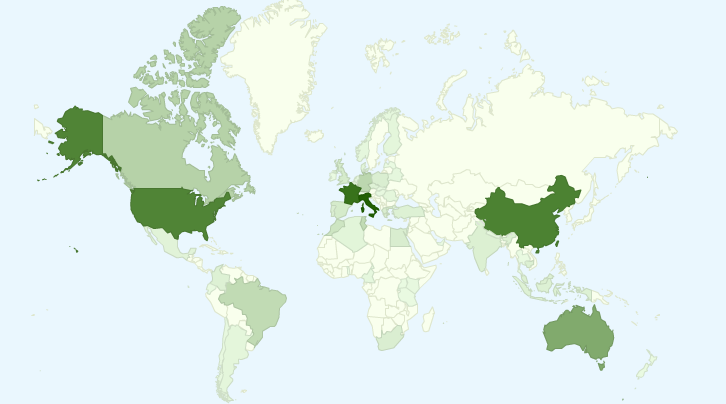
\includegraphics[width=\textwidth]{images/OTB4_download_sourceforge_country_crop.png}
\end{columns}
\end{frame}

\begin{frame}
\frametitle{Success stories}
\vspace{-0.5cm}
\begin{columns}
\column{0.6\textwidth}
\begin{itemize}
\item OTB useful for some of the ORFEO users
\item Used in a large variety of contexts beyond ORFEO now
\item L'OTB a traité avec succès plus de 619 images Pléiades pour le site web RTU,
\item L'OTB fournit beaucoup de fonctions utiles pour la télédétection dans un \textbf{unique outil}
\item L'OTB est (a été) l'unique logiciel open-source compatible avec les images Pléiades (grâce à OpenJPEG)
\item L'OTB égale ou dépasse les outils de l'état de l'art (libre et commercial) pour certaines fonctions:
\begin{itemize}
\item La calculatrice de bandes,
\item La segmentation de scène complètes,
\item La classification à l'échelle d'une scène complète avec un grand choix d'algorithmes,
\item Les ponts entre la télédétection et le systèmes d'information géographique\ldots
\end{itemize}
\item Au delà d'ORFEO, l'OTB est déjà utilisée dans plusieurs projets et logiciels
\end{itemize}
\column{0.4\textwidth}
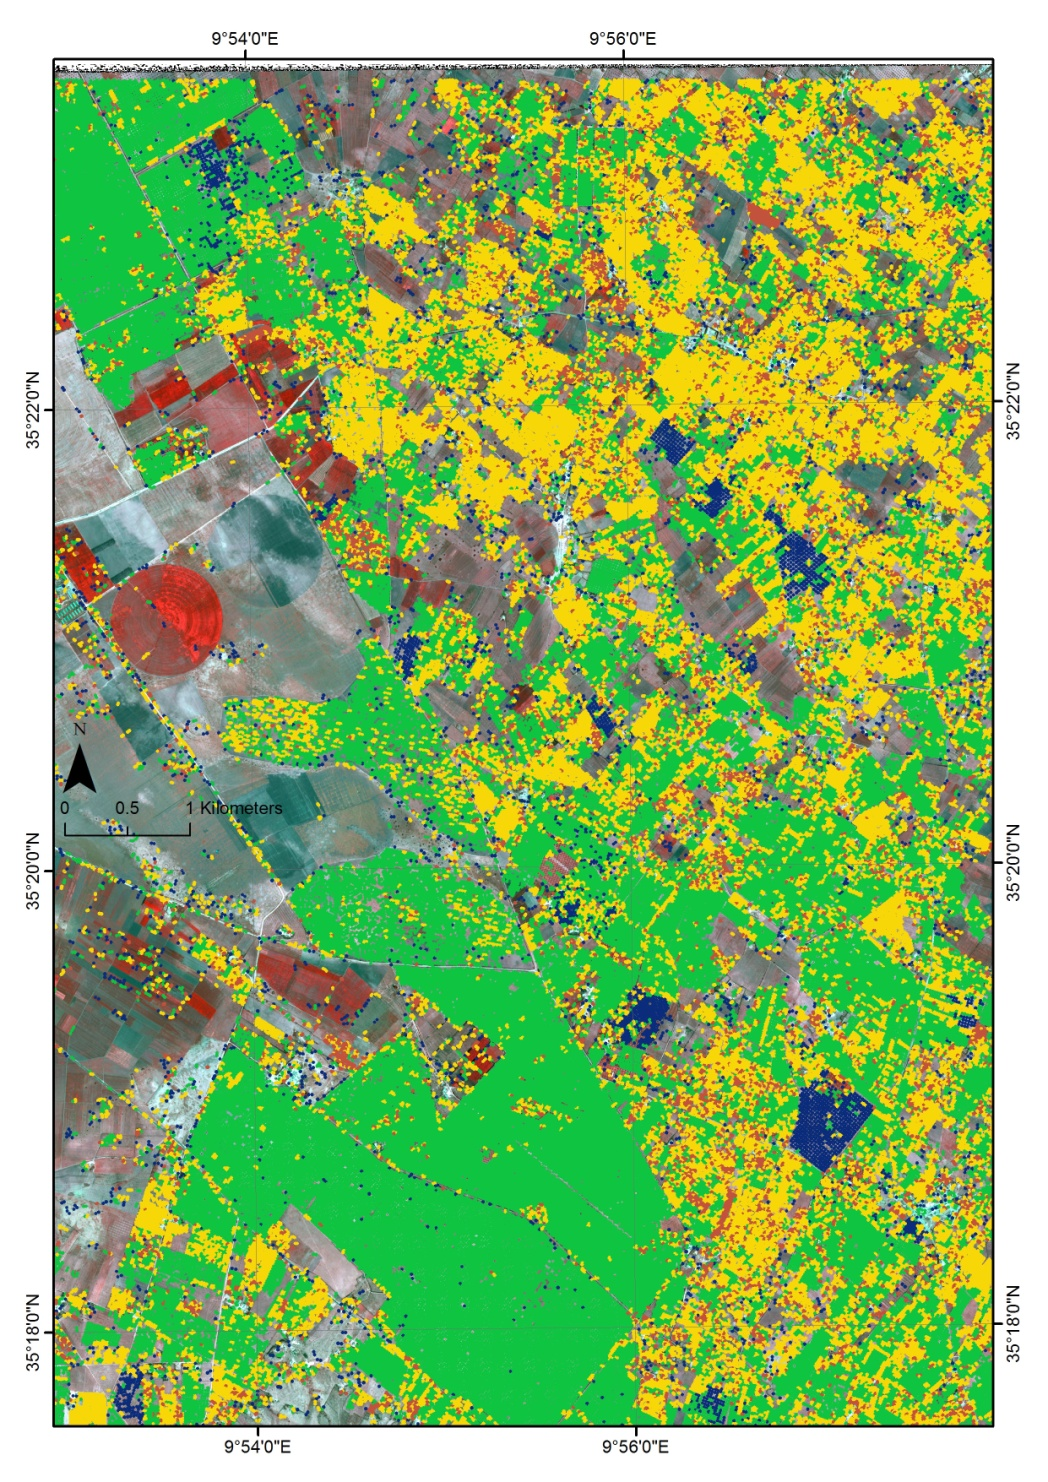
\includegraphics[width=0.9\textwidth]{images/resultats_ird.png}\\
\tiny{Carte thématique à partir d'une segmentation par l'OTB, B. Mougenot~-~IRD}
\end{columns}
\end{frame}

\begin{frame}
\frametitle{Projects and software using OTB}
\begin{columns}
  \column{0.5\textwidth}
  \begin{itemize}
    \item Gnorasi Software (National Technical University of Athens)
    \item Vahine project (hyperspectral processing of astrophysics), IPAG
    \item SEAS project (IRD)
    \item OTB is part of some components for Sentinel-2 and Venus ground segment (CNES and ESA)
    \item TCM research program (ETS Quebec)
    \item Tolomeo FP7 research project (CESBIO)
    \item OTB applications are available through QGIS processing framework
  \end{itemize}
  \column{0.5\textwidth}
  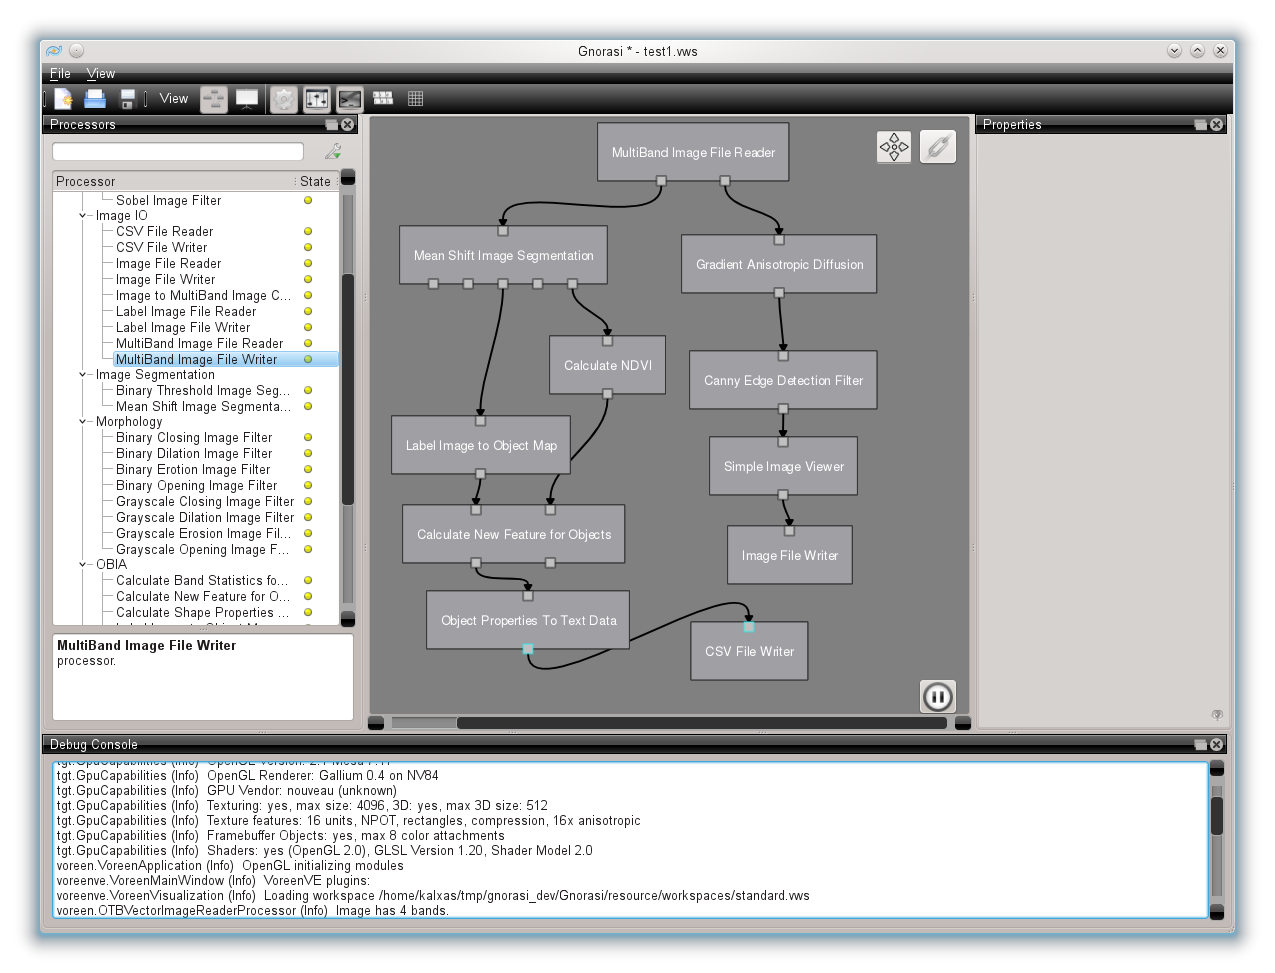
\includegraphics[width=\textwidth]{images/gnorasi2.png}\\
  \tiny{The Gnorasi software}
\end{columns}
\end{frame}

\begin{frame}
\frametitle{A complex system for complex tasks: chaos and side effects}
\begin{center}
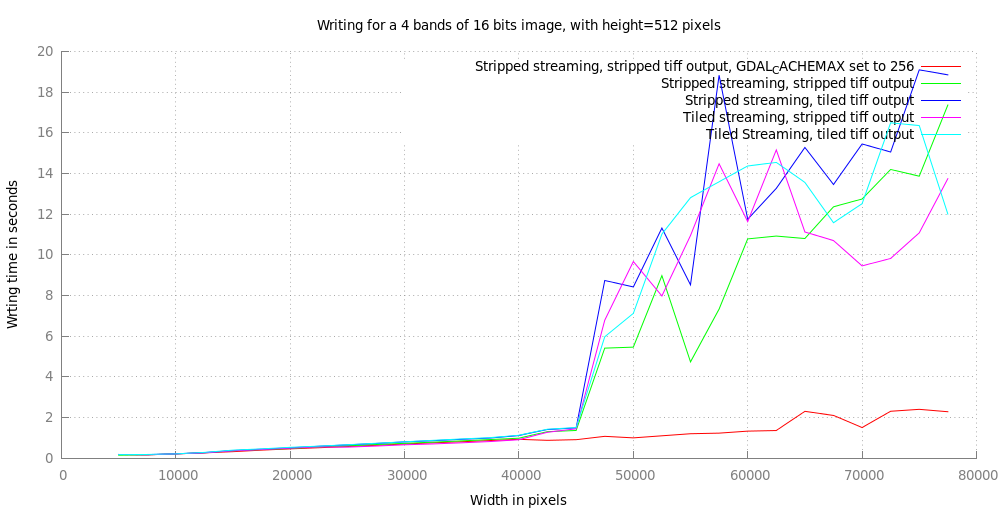
\includegraphics[width=\textwidth]{images/Writing.png}\\
\tiny{Effect of image encoding on image processing}
\end{center}
\end{frame}

\begin{frame}
\frametitle{Support / Help to contribute}
\vspace{-0.2cm}
\begin{block}{General ressources}
\vspace{-0.2cm}
\begin{description}
\item[Site web] www.orfeo-toolbox.org
\item[Wiki] wiki.orfeo-toolbox.org
\item[Blog] blog.orfeo-toolbox.org
\end{description}
\end{block}
\vspace{-0.2cm}
\begin{block}{Documentation and help}
\vspace{-0.2cm}
\begin{description}
\item[Doxygen] \url{http://www.orfeo-toolbox.org/doxygen/}
\item[Guides] Software Guide and CookBook (remote sensing recipes)
\item[Liste utilisateurs] otb-users@googlegroups.com
\item[Liste développeurs] otb-developers@googlegroups.com
\end{description}
\end{block}
\vspace{-0.2cm}
\begin{block}{Suivi rapproché}
\vspace{-0.2cm}
\begin{description}
\item[Que se passe-t-il ?] \url{scrum.orfeo-toolbox.org}
\item[Weather?] \url{dash.orfeo-toolbox.org}
\item[Look at the code?] \url{hg.orfeo-toolbox.org}
\item[Find a bug?] \url{bugs.orfeo-toolbox.org}
\end{description}
\end{block}
\end{frame}

\begin{frame}
\frametitle{Thank you! Any questions?}
\begin{minipage}[t][6cm][t]{\textwidth}
\begin{center}
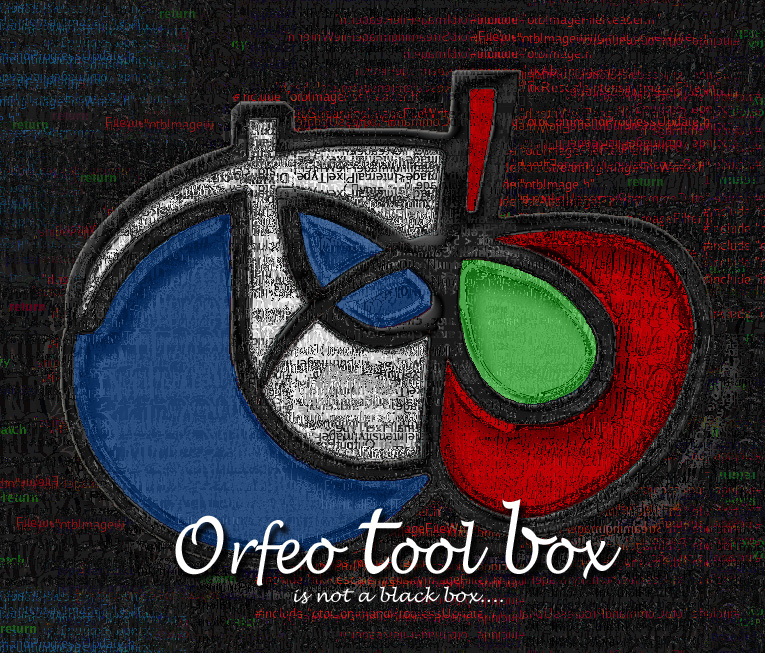
\includegraphics[width=0.7\textwidth]{images/LOGOTB_blackbox.png}
\end{center}
\end{minipage}
\end{frame}

\end{document}
